%\documentclass[man]{apa}
\documentclass{apa}[12pt]

\usepackage{amssymb,amsfonts,amsmath}

\usepackage{times,graphicx,float,bm,subfig}

\setcounter{totalnumber}{1}
\newcommand{\stimulus}[1]{\texttt{#1}}

\setlength{\parskip}{\baselineskip}

% ---------- watermark -----------
\usepackage[firstpage]{draftwatermark}
\SetWatermarkAngle{0}
\SetWatermarkFontSize{0.25cm}
\SetWatermarkVerCenter{1.15cm}
\SetWatermarkLightness{0.5}
\SetWatermarkHorCenter{14cm}
\SetWatermarkText{\shortstack[l]{
Gokaydin, D. Navarro, D. J., Ma-Wyatt, A. and Perfors, A. (2016). The structure \\
of sequential effects. Journal of Experimental Psychology: General, 145, 110-123 \\
http://dx.doi.org/10.1037/xge0000106
}}
\SetWatermarkScale{1}
% -------------------------------

\title{The Structure of Sequential Effects}
\author{\normalsize Dinis G\"okaydin, Danielle J. Navarro, Anna Ma-Wyatt, Amy Perfors}

\affiliation{School of Psychology\\University of Adelaide}

\abstract{There is a long history of research into sequential effects, extending more than one hundred years. The pattern of sequential effects varies widely with both experimental conditions as well as as for different individuals performing the same experiment. Yet this great diversity of results is poorly understood, particularly with respect to individual variation, which save for some passing mentions has largely gone unreported in the literature. Here we seek to understand the way in which sequential effects vary by identifying the causes underlying the differences observed in sequential effects. In order to achieve this goal we perform principal component analysis on a dataset of 158 individual results from participants performing different experiments with the aim of identifying hidden variables responsible for sequential effects. We find a latent structure consisting of three components related to sequential effects - two main and a minor. A relationship between the two main components and the separate processing of stimuli and of responses is proposed based on previous empirical evidence. It is further speculated that the minor component of sequential effects arises as the consequence of processing delays. Independently of the explanation for the latent variables encountered, this work provides a unified descriptive model for a wide range of different types of sequential effects previously identified in the literature. In addition to explaining individual differences themselves, it is demonstrated how the latent structure uncovered here is useful in understanding the classical problem of the dependence of sequential effects on the interval between successive stimuli.}

\acknowledgements{The authors would like to thank Simon de Deyne and Nancy Briggs for valuable comments; also Eric Soetens and Ines Jentzsch for permission to reproduce their data.}

\shorttitle{The structure of sequential effects}
\rightheader{The structure of sequential effects}
\leftheader{The structure of sequential effects}

\begin{document}

\maketitle
\newpage

In everyday life we form expectations about future events. We expect that our employer will pay our salary this month because they paid in previous months. We expect that a traffic light will turn red next because it is currently green. We can form these expectations because our environment possesses spatial and temporal regularities that we can exploit. The fact that we can predict the future to some extent allows us to prepare for it, and react faster to those events we expect. If on the other hand we are surprised by an unusual event we will take longer to adapt and respond to the new situation.

But what if there is no pattern to be found in a sequence of outcomes? Short-lived regularities sometimes occur in a random world; if they do, will people think they have found a pattern or dismiss it as part of a random process? Considerable evidence suggests that humans tend to see patterns even when there is none to be found, and that the way in which we do so is revealing about what we consider to be a meaningful sequence of events. One example of this tendency to find a pattern where it does not exist is the so-called `gambler's fallacy', the erroneous belief often harbored by gamblers that after a repetition of the same outcome an alternation becomes more likely. So for instance after two red numbers in a row when playing roulette, many gamblers will believe that black is more likely to occur next \cite{Nickerson02}. Another example is the belief, despite all evidence to the contrary, held by basketball fans in the `hot hand' phenomenon, i.e. that a player is more likely to score after a series of successful shots \cite{Gilovich85}. In both of these cases the pattern found in the random sequence of events mirrors similar patterns in non-random sequences: the hot hand phenomenon mirrors our (hopefully correct!) expectation that our employer will keep paying our salary, or put simply that the sequence will continue to \textit{repeat} itself; conversely, in the gambler's fallacy there is a tendency to believe the sequence will continue to \textit{alternate}. So in short it seems that the patterns people tend to encounter in a random sequence reflect patterns which are common in world and that are useful in structured environments.


Consistent with the view that humans have a strong tendency to find patterns in randomness are the results of experiments designed to test the effects of a random sequence on human expectations. It has been shown that, when performing a number of different experiments, humans persistently shift their expectations depending on recent sequence, and that this is effect is strongest if the last few trials show a regular pattern \cite{Fernberger20,Jarvik51,Bertelson61,Squires76,Maloney05}. In the most commonly used experimental design, people are given a speeded two alternative force choice (2AFC) task, and {\it sequential effects} are observed: the response time (RT) on any given trial is dependent on the stimulus history over the last few trials \cite{Bertelson61,Falmagne65,Hale67,Laming68,Hale69,Remington69,Schvaneveldt69,Laming69,Kirby72,Kirby76,Soetens85,Cho02,Jentzsch02}. The effect of the sequence can be very strong: in some cases it is stronger than effects caused by the stimulus itself \cite{Kornblum69} and it can alter how the current stimulus is perceived \cite{Maloney05}. Moreover, analogous findings have been observed in event-related potentials (ERPs) measured with EEG \cite{Squires76,Sommer90,Sommer99,Jentzsch02} making the overall topic one that lies at the interface between psychology and neuroscience, and of relevance to both fields.

One somewhat underexplored question pertains to the variability of sequential effects across individuals and across experimental conditions. In this paper we present the results of seven experiments designed to elicit a wide range of possible sequential effect patterns from 158 participants. We use latent variable methods to identify the underlying dimensions upon which these patterns vary, and conclude that there are three distinct components related to sequential effects.

\subsection{Measuring sequential effects}

As noted above, sequential effects are generally measured using a speeded 2AFC task. In a typical experiment subjects are presented with a random sequence of two possible stimuli, denoted \stimulus{X} and \stimulus{Y}, to which they have to respond by pressing the correct button as quickly and accurately as possible. When a response is made the stimulus disappears and after a fixed period of time (the \textit{response-stimulus interval}, RSI), the next stimulus is shown. Mean RT is calculated separately for each possible stimulus history, defined in terms of the current stimulus and the preceding four items. If the current stimulus is \stimulus{X}, and the preceding four had all been \stimulus{Y}, we would denote this sequence as \stimulus{YYYYX}. If the stimuli \stimulus{X} and \stimulus{Y} are in some sense interchangeable it is traditional to treat the stimulus history \stimulus{YYYYX} as equivalent to \stimulus{XXXXY}. In both cases there is a string of {\it repetitions} of the same item followed by an {\it alternation}. We use \stimulus{R} to denote a repetition (i.e. \stimulus{XX} or \stimulus{YY}) and \stimulus{A} to denote an alternation (i.e., \stimulus{XY} or \stimulus{YX}). In this notation, the stimulus histories \stimulus{YYYYX} and \stimulus{XXXXY} both correspond to the sequence \stimulus{RRRA}. A pattern of sequential effects, therefore, is defined in terms of the mean RT for each of the 16 logically possible sequences.

The typical result in the sequential effects literature finds that people are fastest when the most recently presented stimulus is consistent with a regular pattern over recent trials, and slowest when it violates such a pattern. If the last four trials have shown pure repetition pattern (i.e. \stimulus{RRR}) then people will be very fast if that pattern continues (i.e., \stimulus{RRRR}) and slow if it is does not (i.e., \stimulus{RRRA}). Similarly, if the last four stimuli have consistently alternated between the two options, people expect the next item to alternate as well, leading to the finding that response times to \stimulus{AAAA} are fast but response times to \stimulus{AAAR} are slow. However, sequential effects do not occur exclusively when the sequence of events displays a perfectly regular pattern. Any sequence of stimuli will induce some expectations about the next event and this in turn influences reaction times. One way to describe this is to say that any sequence has a \textit{benefit} if the next stimulus is expected and a \textit{cost} if it is not. The benefit of each sequence tends to be a function of how many events \textit{equal to the last} it includes. For instance, reaction times tend to be faster to \stimulus{ARRR} than to \stimulus{AARR} because more repetitions happened before the last \stimulus{R} in the former case. In addition, more recent events have a greater influence on expectations, e.g. reaction times will be shorter to \stimulus{AARR} when compared to \stimulus{RAAR}. Therefore, a simplified way to understand the influence of the previous sequence is to consider that each event -- \stimulus{A} or \stimulus{R} -- \textit{primes} subjects to expect the same event, and that the strength of this priming effect decays across trials, so that recent events have a much stronger influence on people's expectations.

To visualize a pattern of sequential effects, it is traditional to plot the mean RTs in a figure similar to Figure~\ref{soetens_rsi}. The left side of the plot shows all sequences ending with an \stimulus{R} and the right half those ending with an \stimulus{A}. Within each half, the sequences are ordered by increasing expected cost if the last event is a repetition, or conversely increasing benefit if it is an alternation. Thus the traditional ``cost-benefit'' view of sequential effects would tend to produce an inverted-V shape when plotted in the usual way \cite<e.g.>{Soetens85,Cho02}. In practice, however, considerable deviations to the ideal cost-benefit scenario exist. For instance, a ``pure'' cost-benefit scenario would produce a symmetric plot, yet in practice this is not always observed. One important way in which results vary is with respect to whether overall reaction times are faster to repetitions or to alternations; in the former case we speak of a repetition bias or of a preference for repetitions, and similarly for alternations.


More generally, there are two main sources of variation in sequential effects: experimental and individual. Firstly, sequential effects depend on experimental parameters, and in particular the response-stimulus interval; secondly, substantial individual differences are observed even if experimental conditions are held fixed. In some cases these differences -- both experimental and individual -- are relatively small, consisting of a slight repetition or alternation bias on what is otherwise a clear cost-benefit pattern. However, in other cases the pattern of results is entirely different and no longer easily interpretable in terms of any form of priming or pattern detection. In the following sections we briefly discuss these variations.

\subsection{Experimental differences}

\begin{figure}[t]
\centering
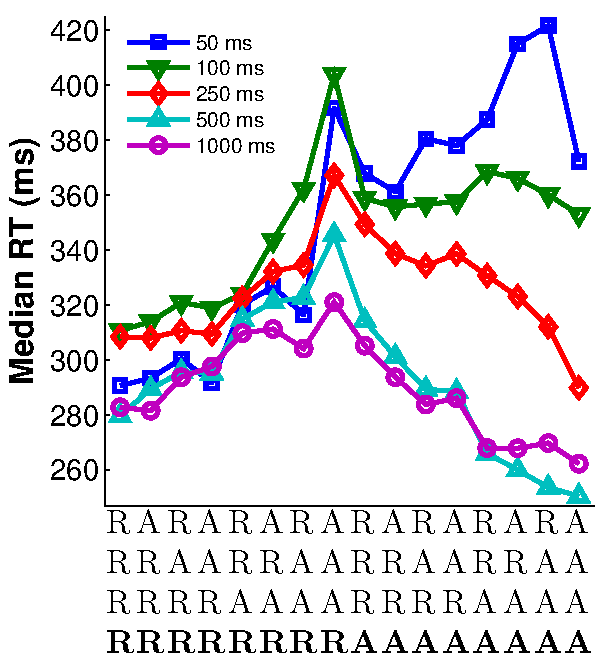
\includegraphics[width=.5\textwidth]{soetens_rsi_plot.pdf}
\caption[Dependence of sequential effects on the RSI]{The dependence of sequential effects on the RSI. Adapted from \protect\citeA{Soetens85} with permission. Each line corresponds to a different set of 10 subjects which performed the same experiment with a different RSI value. Other than the choice of RSI, the experimental protocol was exactly the same, with two horizontally displaced dots as stimuli, similar to Experiment 3 (see Method section).}\label{soetens_rsi}
\end{figure}

A cost-benefit pattern of sequential effects -- the inverted-V -- is often observed in experiments conducted with a long RSI (see Figure \ref{soetens_rsi}; 1000, 500 and 250 ms RSI) and this is usually considered to reflect an expectation-based mechanism, often referred to as \textit{subjective expectancy} \cite{Kirby76,Soetens85}. In contrast, when a short RSI -- under 100 ms -- is used a substantially different pattern of sequential effects is usually observed, displaying an approximately monotonic increase in reaction time when plotted the classical way (see Figure \ref{soetens_rsi}; 50 ms RSI). This was originally considered to reflect a unidirectional effect of the previous sequence, which would induce faster or slower reaction times irrespective of what the last event is, leading to this pattern of results being coined \textit{benefit-only} \cite{Laming68,Soetens85}.\footnotemark{} Given that it no longer seemed compatible with expectations generated by the pattern in the sequence, the benefit-only pattern of sequential effects was ascribed to a low-level mechanism termed \textit{automatic facilitation} \cite{Soetens84,Soetens85}. As the RSI is shortened, sequential effects gradually change from a cost-benefit to a benefit-only pattern (see Figure \ref{soetens_rsi}), and as the classical theory goes this would reflect a gradual transition between subjective expectancy and automatic facilitation.

\footnotetext{We will not go into much detail about automatic facilitation and how it could have a unidirectional effect on reaction times. For the purposes of this study `benefit-only' should be taken as a label useful in referring to the pattern of sequential effects often observed when the RSI short.}

\begin{figure}[t]
\centering
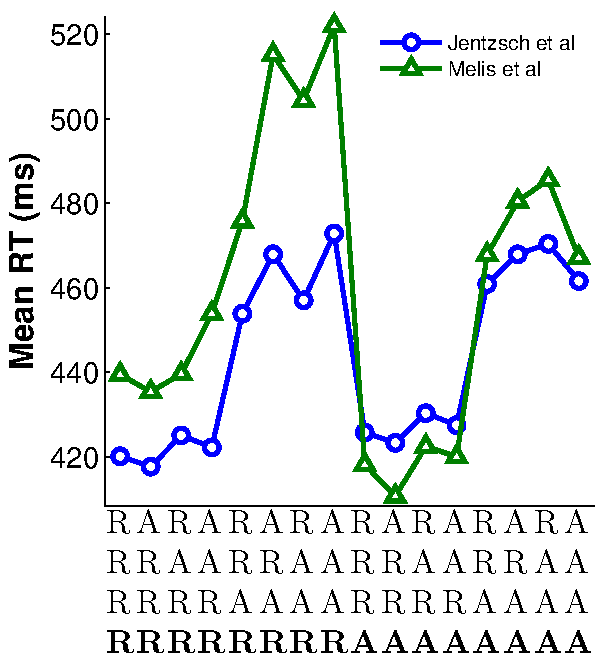
\includegraphics[width=.5\textwidth]{melis_jentzsch.pdf}
\caption[Unusual patterns of sequential effects]{Unusual patterns of sequential effects. The results of two experiments are shown: the second experiment conducted by \protect\citeA{Jentzsch02} and results from an elderly group of subjects included in \protect\citeA{Melis02}. Notice the approximately two-tiered pattern of results depending on whether the second-to-last event was a repetition or an alternation, irrespective of the last event. Both experiments were standard 2AFCs with separate dots as stimuli and both were conducted with a 50 ms RSI; the experiment by \protect\citeA{Jentzsch02} was considerably longer both in terms of total trials (3960 vs 1560) and number of trials in one block (330 vs 120). Adapted with permission from the authors.}\label{melis_jentzsch}
\end{figure}

Most empirical results fall somewhere along the continuum between the cost-benefit and benefit-only patterns sequential effects \cite<e.g.>{Vervaeck80,Soetens85,Cho02,Jentzsch02,Gokaydin11}. However, there are at least two experiments in which a qualitatively different pattern of sequential effects was obtained \cite{Jentzsch02,Melis02}. In both cases (shown in Figure \ref{melis_jentzsch}) results point to a dependence of reaction times on the \textit{second-to-last} event independently of the last one \cite{Jentzsch05}.\footnotemark{} One hint of what may be behind this unusual pattern of results comes from the work of \citeA{Melis02} in which two groups, one of elderly and one of young subjects, performed the same experiment. When the RSI was long (1000 ms) both groups displayed a typical cost-benefit pattern; when the RSI was short (50 ms) the young group displayed a benefit-only pattern of sequential effects as expected but the elderly group produced the results shown in Figure \ref{melis_jentzsch}. \citeA{Melis02} suggest that the underlying variable responsible for the differences observed between age groups is processing speed, of which age is a close correlate.

\footnotetext{Note that under normal circumstances reaction times depend on the second-to-last event too, but \textit{conditional} on the last one. In this case it is as if the last event did not happen.}

In addition to the RSI, several other experimental parameters influence sequential effects. These include stimulus-response compatibility \cite{Bertelson65,Soetens85}, different stimuli \cite<e.g.>{Hale67,Soetens85,Cho02} or different response schemes such as if one or two fingers are used to respond \cite{Hannes68,Gokaydin11}, among others. However, the effects of most of these experimental manipulations again seem to fall along the continuum between a cost-benefit and benefit-only patterns, something which was described in great detail for the case of response-stimulus compatibility \cite{Soetens85}. So in order to describe the full spectrum of possible sequential effects one could invoke the continuum in Figure \ref{soetens_rsi} together with the less common results shown in Figure \ref{melis_jentzsch}.

\subsection{Individual differences}

\begin{figure}
\centering
\begin{tabular}{ccc}
\multicolumn{3}{c}{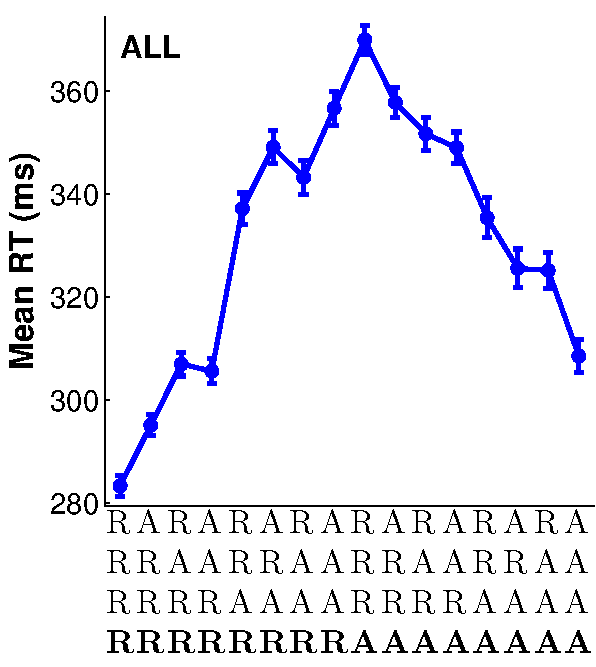
\includegraphics[width=0.35\textwidth]{cho_rsi_500ms.pdf}} \\

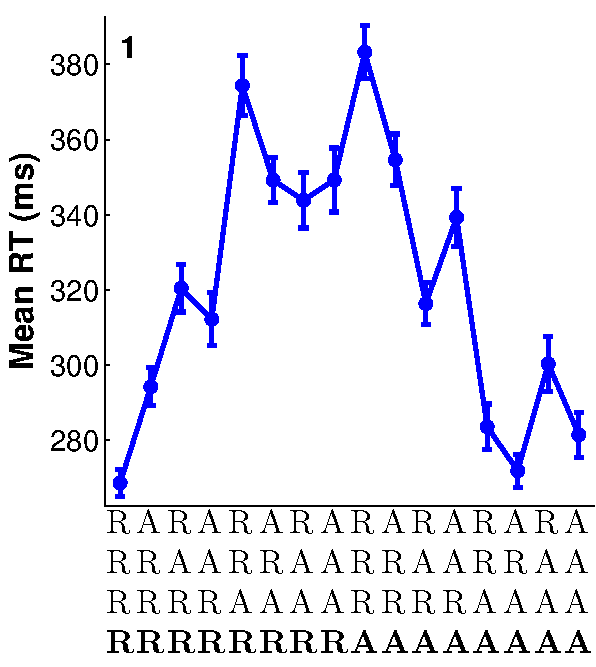
\includegraphics[width=0.25\textwidth]{subject1_500ms.pdf}\label{individual1}
   & 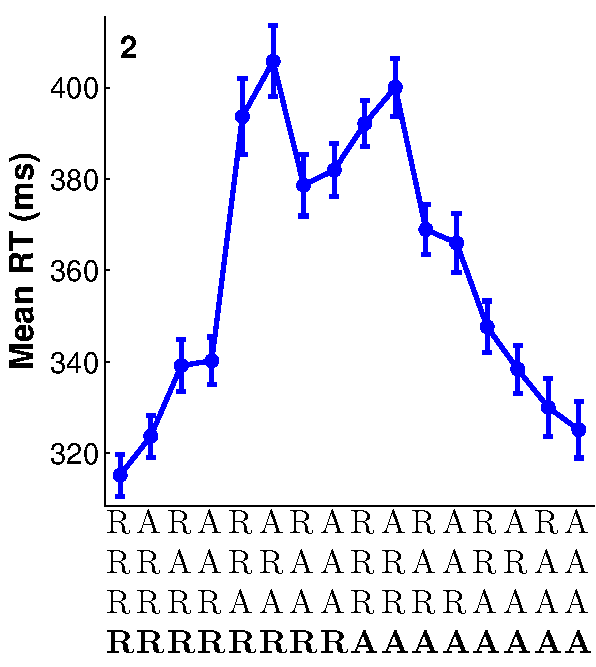
\includegraphics[width=0.25\textwidth]{subject2_500ms.pdf}\label{individual2}
   & 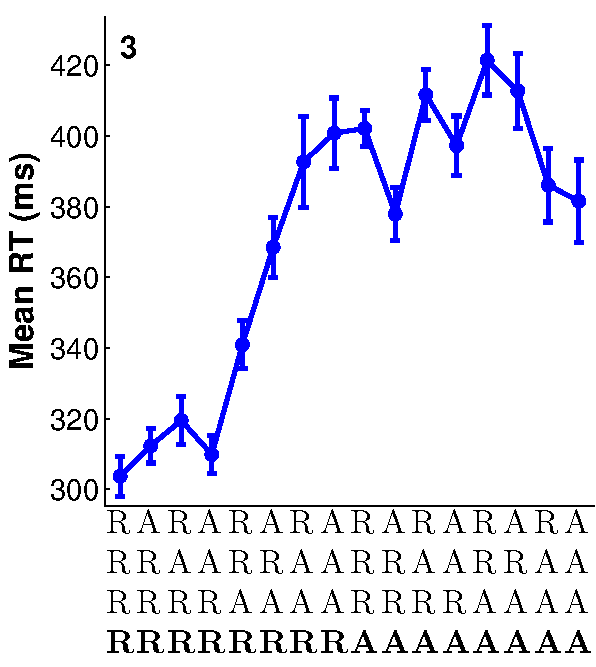
\includegraphics[width=0.25\textwidth]{subject3_500ms.pdf}\label{individual3}\\
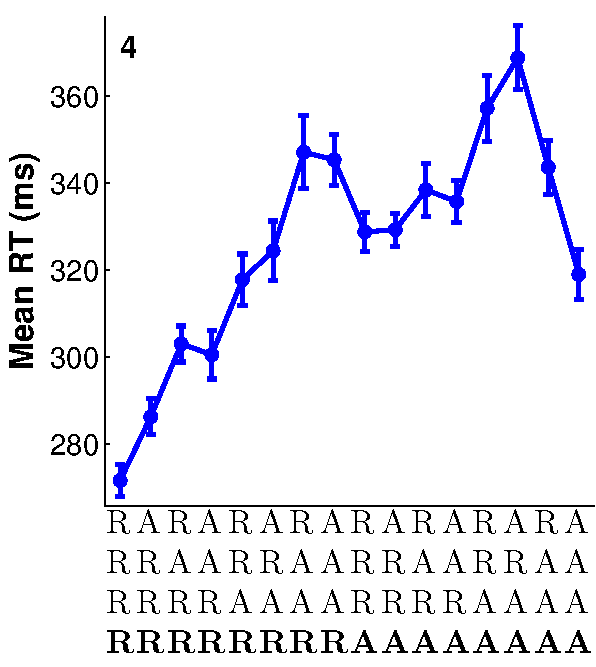
\includegraphics[width=0.25\textwidth]{subject4_500ms.pdf}\label{individual4}
   & 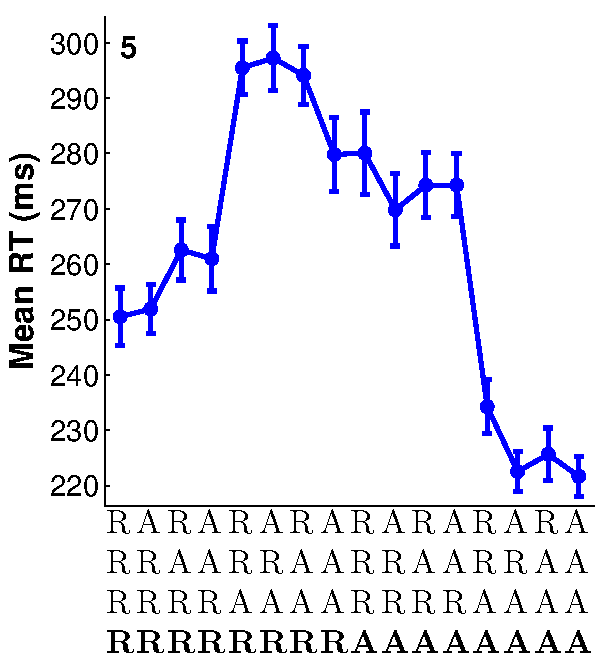
\includegraphics[width=0.25\textwidth]{subject5_500ms.pdf}\label{individual5}
   & 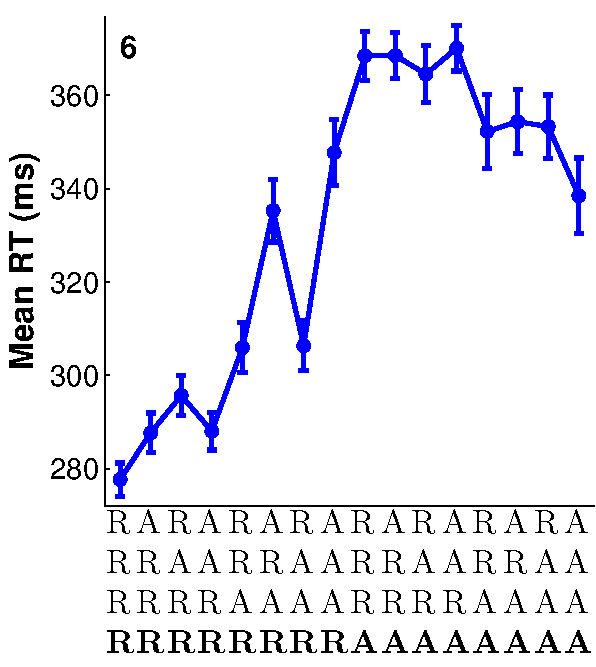
\includegraphics[width=0.25\textwidth]{subject6_500ms.pdf}\label{individual6}\\
\end{tabular}
\caption[Individual differences for the same experimental conditions]{Individual differences for the same experimental conditions. Top panel (ALL) shows the average RT pattern of all six subjects which performed Experiment 1 with a 500 ms RSI. The bottom panels (1-6) show the results of the same six individuals separately. Note that while the average pattern shows a clear cost-benefit pattern with only a slight repetition bias, the individual subjects that make it up display marked deviations from the average pattern. Error bars show the standard error of the mean.}\label{individual_subjects}
\end{figure}

All the results discussed so far are averages taken across a set of participants. However, considerable individual differences are usually present for the same experimental conditions, but are not typically considered in much detail. Several mentions of individual differences in sequential effects exist in the literature, but these are usually limited to a passing observation that some individuals display a preference for repetitions and others to alternations \cite{Arons32,Bertelson65,Kornblum69,Kirby76}.

The main reason why individual differences in sequential effects are usually hidden from view is that it experimental results are generally presented by averaging across participants. This practice may be somewhat misleading. To foreshadow some of our own results, Figure \ref{individual_subjects} shows a sample of the data collected for this work illustrating individual variation for the same experimental conditions (Experiment 1, 500 ms RSI). The average pattern of results across all subjects (Figure \ref{individual_subjects}, top panel) displays a typical cost-benefit pattern, but most individual subjects reveal substantial deviations to such a pattern. This is actually the rule rather than the exception, with similar levels of variation in all experiments reported here. Notably, the way individual subjects differ from each other for a \textit{fixed} RSI is similar to the way in which collective average results vary with RSI (see Figures \ref{soetens_rsi} and \ref{rsi_scan}). For instance, the pattern of results of subject 3 in Figure \ref{individual_subjects}, which was obtained with an 800 ms RSI, is similar to the benefit-only pattern of sequential effects usually observed when a short RSI is used (see Figure \ref{soetens_rsi}; 50 ms data). These similarities indicate that not only are individual differences unlikely to be due to noise but also that they may be related to the dependence of sequential effects on the RSI.

If individual differences are meaningful, then exploring the patterns of covariance across multiple subjects may be of use in identifying latent variables contributing towards sequential effects. However, it is also important that such an analysis be informed by what is already known about the possible mechanisms underlying sequential effects. With that in mind, we turn to a brief discussion of the evidence suggesting that there are distinct processing stages involved in sequential effects, as these these are likely to play a role in the differences observed, both across individuals as well as across experiments.

\subsection{Processing stages in sequential effects}

\begin{figure}[t]
\centering
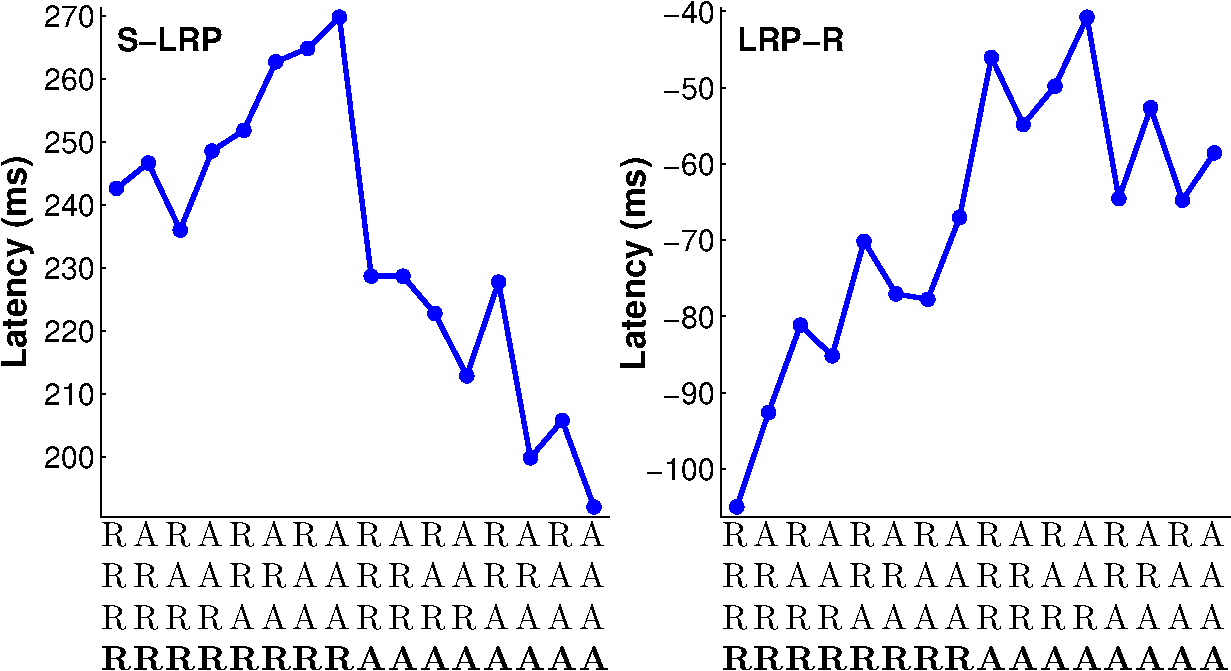
\includegraphics[width=.7\textwidth]{slrp_lrpr.pdf}
\caption[S-LRP and LRP-R]{Reaction time decomposition of sequential effects performed by \protect\citeA{Jentzsch02}. The time between stimulus onset and the rise of the lateralized readiness potential (LRP) is shown on the left plot (S-LRP); the right plot shows the time between the rise of LRP and the moment a response is made (LRP-R). The LRP peaks just before a response is made and is more negative contra-laterally to the hand which will be use to respond. The time of LRP onset is defined as the moment it reaches a threshold amplitude. Adapted with permission from the author.}\label{slrp_lrpr}
\end{figure}

There has been some debate in the literature as to whether sequential effects are primarily related to the stimuli themselves, the associated responses, or both \cite{Bertelson65,Soetens98}. Overall, evidence points to the fact that both stimuli and response related effects are involved in sequential effects, but there is some neurophysiological evidence that helps to disambiguate the two.
\citeA{Jentzsch02} conducted a study of sequential effects in the lateralized readiness potential (LRP) measured with EEG. The LRP is a negative shift in electrical potential just before a response, and located in the pre-motor cortex area contra-lateral to the hand which will be used to respond. It is thought that the time after the occurrence of the LRP is exclusively due to motor processing \cite{Leuthold96}. Therefore, by measuring the time between stimulus onset and the rise of LRP signal (S-LRP) and the time between LRP and the moment a response is made (LRP-R) the authors sought to measure pre-motor and motor processing time respectively.\footnotemark{} Further, by measuring S-LRP and LRP-R as a function of the the sequence of events in a traditional 2AFC, the relative contribution of motor and pre-motor processing stages towards sequential effects was estimated (see Figure \ref{slrp_lrpr}).

\footnotetext{Note that S-LRP + LRP-R = RT for each trial. This is not necessarily true for the average S-LRP and LRP-R calculated from multiple subjects and shown in Figure \ref{slrp_lrpr}, but in practice a sum of the average S-LRP and LRP-R is very close to the average RT pattern.}

It is natural to suppose that the pre-motor stage reflects the processing of stimuli and the motor stage the processing of responses. In fact, there is some empirical support for this association from experiments which attempt to selectively remove the influence of stimuli on the one hand, and of responses on the other hand, from sequential effects. In an experiment where the effect of responses is removed a pattern of reaction time results is obtained which is very similar to S-LRP, the pre-motor processing component \cite{Maloney05}. Conversely, in an experiment where the effect of the stimuli is removed, a pattern similar to LRP-R is obtained \cite{Wilder13}. That selectively removing the influence of stimuli and of responses produces reaction time results similar to LRP-R and S-LRP in isolation provides support for an association between the pre-motor stage and the processing of stimuli on the one hand, and the motor stage and the processing of responses on the other hand.

If separate processing stages contribute towards sequential effects it is possible that these play a role in producing different patterns of results. However, it is not clear how the relative contribution of either processing stage changes both when the RSI is varied as well as for different individuals. One possibility is that stimulus and response processing will always display contributions similar to S-LRP and LRP-R, with only the \textit{magnitude} of one or the other changing under different circumstances. Mathematically speaking, this amounts to suggesting a linear combination of S-LRP and LRP-R -- as shown in Figure \ref{slrp_lrpr} -- as a preliminary descriptive model for sequential effects. Crucially, this hypothesis hinges on the relative contribution of stimulus and response processing remaining fixed when the RSI is varied, as well as across different individuals. However, baseline problems prevented the use of the LRP method for a short 50 ms RSI \cite{Jentzsch02}. With respect to how stimulus and response processing would vary across individuals, no such data exists as yet. So in short it is not known how the relative contribution of the two processing stages of sequential effects changes.

Some indirect evidence for the linear combination hypothesis exists and stems from the fact that such a model does a good job of describing individual results, particularly when the RSI is long, and not only those subjects which display a cost-benefit pattern expected from a simple sum of S-LRP and LRP-R. Furthermore, as discussed above, patterns similar to both S-LRP and LRP-R can be isolated in reaction time data under different experimental circumstances to those under which the EEG processing measurements were done. Collectively, this evidence points to the fact that the patterns displayed by S-LRP and LRP-R are meaningful beyond the set of experimental circumstances in which they were first identified.

\subsection{Summary and goals}

In this work we infer latent variables involved in sequential effects by analyzing the patterns of covariance across individual reaction time data, using a dataset consisting of 158 participants across 7 experiments and 4 RSIs. Moreover, we attempt to relate this latent structure to the two proposed processing stages of sequential effects discussed above. In doing so, we do not propose a theory of individual differences in sequential effects, but instead aim to shed light on the nature of sequential effects by understanding the dimensions upon which it is possible for a sequential effects pattern to vary, across individuals and experiments.

\section{Method}

\subsection{Participants}

158 participants performed several experiments which differed in the type of stimuli used and the response scheme. For each experimental design, four values of RSI were tested -- 50, 250, 500 and 800 ms -- except in the case of Experiment 2 with a 50 ms RSI due to a technical error. The majority of participants (149/158) were undergraduate students from the University of Adelaide and were awarded course credit for performing the experiment. A few participants were recruited among University staff and graduate students as well as the surrounding community (9/158). All participants gave their informed consent to taking part in the experiments. Table \ref{table_subjects} shows the number of participants used per experiment and RSI. Three participants performed two different experiments. Two of the authors (DG and AP) are among the participants, having taken part in only one experiment each.

%\begin{table}[t]
%\centering
%\caption[Number of participants per experiment and RSI]{Number of participants per experiment and RSI}
%\label{table_subjects}
%\begin{tabular}{c|cccccccc|c}
%Experiment & 50ms & 100ms & 250ms & 400ms & 500ms & 700ms & 800ms & 1000ms & Total
%\\ \hline \\
%1    & 4 & 0 & 5 & 0 & 6 & 0 & 7 & 5 & 27\\
%2    & 0 & 5 & 6 & 0 & 6 & 0 & 5 & 0 & 22\\
%3    & 10 & 0 & 5 & 0 & 5 & 0 & 10 & 5 & 35\\
%4    & 5 & 0 & 5 & 5 & 5 & 0 & 5 & 0 & 25\\
%5    & 5 & 0 & 4 & 0 & 6 & 0 & 8 & 0 & 23\\
%6    & 8 & 0 & 5 & 7 & 5 & 7 & 5 & 4 & 41\\
%7    & 8 & 0 & 5 & 0 & 5 & 0 & 5 & 0 & 23\\
%8    & 0 & 0 & 0 & 0 & 0 & 0 & 7 & 0 & 7\\
%9	 & 0 & 0 & 0 & 0 & 0 & 0 & 9 & 0 & 9\\
%\\ \hline \\
%Total & 40 &	5 & 35 & 12 & 38 & 7 & 61 & 14
%
%\end{tabular}
%\end{table}

\begin{table}[t]
\centering
\caption[Number of participants per experiment and RSI]{Number of participants per experiment and RSI}
\label{table_subjects}
\begin{tabular}{c|cccccccc|c}
Experiment & 50ms & 250ms & 500ms & 800ms & Total
\\ \hline \\
1    & 4 & 5 & 6 & 7 & 22\\
2    & 0 & 6 & 6 & 5 & 17\\
3    & 10 & 5 & 5 & 10 & 30\\
4    & 5 & 5 & 5 & 5 & 20\\
5    & 5 & 4 & 6 & 8 & 23\\
6    & 8 & 5 & 5 & 5 & 23\\
7    & 8 & 5 & 5 & 5 & 23\\
\\ \hline \\
Total & 40 & 35 & 38 & 45 & 158

\end{tabular}
\end{table}

\subsection{Experiments}

\begin{table}[t]
\centering
\caption[Summary of experimental designs]{Summary of experimental designs}
\label{table_experiments}

\begin{tabular}{cccc}
%\multicolumn{1}{c}{\bf PART}  &\multicolumn{1}{c}{\bf DESCRIPTION}
Experiment & Stimuli & Response & Notes
\\ \hline \\
1   & $\lbrace \text{o},\text{O}\rbrace$ & Index and middle finger &\\
2   & $\lbrace \text{o},\text{O}\rbrace$ & Both index fingers &\\
3   & Two horizontal dots & Both index fingers  &\\
4   & Two horizontal dots & Both index fingers & Incompatible mapping\\
5   & Two horizontal dots & Index and middle finger &\\
6   & Two vertical dots & Both index fingers &\\
7	& Two vertical dots & Both index fingers & Stimulus flashes for 50ms\\
\end{tabular}

\end{table}

Data from seven different variations of a 2AFC was used in this work. These variants were originally designed in order to test the impact of different experimental factors on sequential effects. Although conducted as separate experiments they share a common procedure and will be analyzed together.\footnotemark{} The experiments differed in two main respects: the stimuli used and response scheme used. Stimuli consisted either of two separate dots (aligned vertically or horizontally), or a lower- and upper-case `o'. Response schemes consisted of using the index and middle finger of the dominant hand or using both index fingers. Additional respects in which experiments differed were response-stimulus compatibility, i.e. whether response buttons were assigned to the stimuli on the same side or on the opposite side, and whether a stimulus was quickly flashed or if it remained on screen until the moment a response was made. Table 2 summarizes the differences between the experiments; for each set-up, different groups of subjects used a particular RSI value, which was held fixed throughout the experiment.

\footnotetext{Note that the between-subjects manipulations mean that the interpretation of our analyses is slightly different from an individual differences study, in which all manipulations are within-subject. This means that the resulting variation in sequential effects is caused by both experimental and within-subject variations. Given that our goal is to explore the range of what sequential effects patterns are {\it possible} across different people and different tasks (something that is not currently well-understood), this additional variability is not inherently problematic. The important thing is that care must be taken not to attribute any specific pattern of performance solely to the individual subject: it depends on both the person and the task.}

\subsection{Procedure}

Subjects sat approximately 60cm away from the computer screen, inside a darkened room. The stimuli were white, approximately 3cm tall, and displayed against a gray background using Psychophysics Toolbox 3 and Matlab r2008a on a 17" Macintosh MacBook Pro. For responses, a Cedrus RT-530 response time box was used, which has one central round button surrounded by four rectangular buttons. The RT box was placed to the right of the screen if the subject was right-handed, to the left if left-handed, and in front of it if the subject was using both hands. In experiments where only one hand was used the subject was asked to use the dominant hand. Responses were made by pressing one of two buttons, each corresponding to a particular stimulus. Subjects were instructed to respond as quickly and accurately as possible by pressing the button assigned to the stimulus shown. If the stimuli differed in shape (Experiments 1, 2) rather than position on the screen (Experiments 3 through 7) the assignment of response button to stimulus was alternated with each new subject. Experiment 4 differed from the rest in that an incompatible mapping was used, i.e. the left side button was used to respond to the right side dot and vice-versa.

Stimuli remained on the screen until a response was made, except for Experiment 7 in which stimuli flashed for 50 ms and then disappeared. In either case, once a response was made the RT and the button pressed were recorded. After a fixed period of time termed the response-stimulus interval (RSI), the next stimulus appeared. The only feedback was a beep whenever a button was pressed. The accuracy and precision of RT measurements were both estimated to be on the order of one millisecond. Only trials where subjects responded correctly were included in the analysis.

All experiments consisted of 13 blocks of 120 trials each, with a short (approximately 1 min) break in between each block and a longer break (5 to 10 min) after the seventh block. Subjects were given one block of training before beginning except in Experiment 4 where the added difficulty required two such blocks. Data from training blocks was not used in the analysis. Sequences were generated randomly for each subject, with the constraint that the frequency of both stimuli be equal.

\subsection{Data analysis}

\subsubsection{Variables}

For each participant, the RT at each point in the sequence was recorded; trials where an error was made were discarded, as were the first four trials in each block. The RT values were then grouped according to preceding sequence of 5 stimuli, including the one being responded to, for a total of sixteen groups. In light of the fact that the RT distribution is always positively skewed, we took the logarithm of all values in each bin \cite{Ratcliff93}. Outliers beyond two standard deviations of the mean of the log transformed RTs were. Finally, the RTs were transformed back to linear scale and thir mean was calculated. Each individual is therefore represented in the analysis by a 16-long array of mean RT values, each corresponding to one of sixteen possible five-long sequences of stimuli or, equivalently, four-long histories of repetitions and alternations.

\subsubsection{Inferring latent structure}

Principal component analysis (PCA) was used in order to identify latent structure. This may seem surprising, given that factor analysis is usually the preferred method for exploratory latent variable modelling \cite<e.g.>{fabrigar1999evaluating}. The reason for preferring PCA is that in our data the communalities are very nearly 1, and factor analysis is not designed for this situation nor is robust when it arises, producing Heywood cases.\footnote{It is in fact the explicit recommendation made by SAS that under these circumstances PCA should be used in place of factor analysis \cite[pp 2105-2106]{SAS2010}.} The extremely large communality is not accidental, and arises as a natural consequence of our experimental design. Because each measured variable is the average taken across a very large number of individual RTs, the (quite small) measurement error is of negligible size relative to the (quite large) variations across subjects, experiments and stimulus histories. In the absence of measurement error, the only way for communalities to be smaller than 1 is if there exist {\it specific factors} in addition to common factors, where specific factors refer to substantive effects that apply only to one variable. Yet it makes very little theoretical or empirical sense to expect any such factors to exist: it is tantamount to the claim that there is something so special about the specific stimulus history \stimulus{AARR} that is not explained by the priming effects of alternations or repetitions, and is so unique that it is not common to \stimulus{ARRR}, \stimulus{AAAR}, \stimulus{RRAA} or any of the other stimulus histories for which mean RT could be measured. There is nothing in sequential effects literature that gives any reason to expect such effects to exist. Given the above, the structure of our data is such that {\it all} covariation should be due to the common factors, and it is precisely this assumption that is built into PCA but inconsistent with the factor analysis model \cite<again, see>{fabrigar1999evaluating}.


We refer to the latent variables identified in this fashion as the `components' of sequential effects. Each component is attributed a set of \textit{coefficients}, one for each of the sixteen observed variables, which can be interpreted as correlation coefficients or as the variance of each observed variable by the corresponding latent component. The set of coefficients for a particular component will be referred to as its `coefficient pattern', by analogy with factor patterns in factor analysis. In addition, each individual participant is attributed a set of \textit{scores}, one for each component retained, which reflect the relative contribution of each component for each individual's results. Finally, the latent components will be denoted as C1, C2, C3 and so on, the numbering referring to the order in terms of variance explained. Before rotation, the first four components we chose to retain explain 78\%, 12\%, 5\% and 1.26\% of variance, and it will shortly become obvious why we chose to keep all four. Collectively, these four variables explain over 96\% of the variance, consistent with our expectation that communalities would be extremely high.

\subsubsection{Component rotations}

Although the probabilistic model underpinning PCA is appropriate for our data, there is no inherent reason to think that the four unrotated components correspond to any theoretically meaningful constructs. Fortunately, the existing literature provides some hints as to what would count as a meaningful latent variable. If the S-LRP and LRP-R components discussed previously genuinely do correspond to distinct processing stages, then they are natural candidates for latent components. With that in mind, targeted procrustes rotations will be used in an attempt to find the best match possible between latent components and empirical data, instead of more traditional methods such as varimax which result in a relatively arbitrary solution \cite{Gorsuch83}.\footnote{Oblique rotations are used throughout except when estimating the variance explained by each component, in which case orthogonal rotations are be used instead. The reason for this is that estimating the variance explained by correlated components is analytically intractable. In any case, the orthogonal solution is very similar to the oblique one and so the variance estimates are expected to be reasonably accurate.}

Four components were retained and so four targets are necessary for the procrustes rotation, one for each component, C1 to C4. The four targets were were, in order: a constant vector to represent mean response time (C1); the S-LRP pattern to represent early processing (C2); the LRP-R to represent late processing (C3); and the reaction time results of the second experiment performed by \citeA{Jentzsch02} shown in Figure \ref{melis_jentzsch} to capture the unusual pattern sometimes seen at very short RSIs (C4). All targets were $z$-scored in order to scale and center them.

\section{Results}

\begin{figure}[t]
\centering
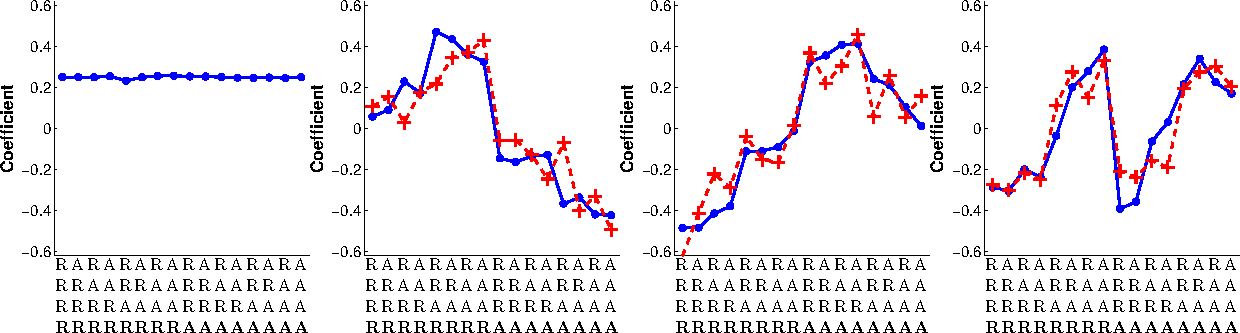
\includegraphics[width=1\textwidth]{component_fits_oblique.pdf}
\caption[Latent structure of sequential effects.]{Latent structure of sequential effects. Solid blue lines plot the coefficient patterns of the first four components identified with PCA after an oblique targeted rotation (see main text for details). Dashed red lines show the targets used for the rotation of the latent components, linearly fit to the respective coefficient patterns. Note that the first component C1 simply captures variation in mean RT across participants and experiments and is not a form of sequential effect. The components are ordered from left to right by amount of variance explained: 78\%, 8.3\%, 7.88\% and 2.4\% respectively for C1 to C4. $R^2$ values for the fits to C2, C3 and C4 are 0.81, 0.88 and 0.84 respectively.\label{component_fits}}
\end{figure}

As illustrated by Figure~\ref{component_fits}, the rotated components provide a very good match to the four target patterns, and as such it seems reasonable to attach meaningful interpretation to them. Individual differences in mean RT (i.e., C1) is the primary dimension upon which ``sequential effects'' patterns can vary, accounting for 78\% of the overall variance. However, given that this pattern merely acts to shift all RTs up or down independent of the stimulus history, it is not a sequential effect. Of more theoretical interest is the fact that the patterns corresponding to early and late processing (C2 and C3) capture most of the remaining variance, at 8.3\% and 7.8\% of the variance respectively. Finally, the second-to-last pattern (C4) found by \citeA{Melis02} and \citeA{Jentzsch02} captures a small proportion of the variance (1.9\%), though as discussed later there are systematic patterns in our data regarding when C4 is influential. Although the raw percentages are small (i.e., 8.3\%, 7.88\% and 2.4\% do not seem very large) this is a consequence of the very large effects of overall mean RT. When the individual subject data are normalized to have the same mean prior to the analysis, these numbers become 38.2\%, 35.5\% and 11.5\% respectively for C2, C3 and C4. These numbers are a better representation of the relative contribution of each component to the sequential effects.


\subsection{Variation across experiments}

We ran analyses of the latent structure across the different experiments analogous to the analyses presented at separate RSI values discussed below, and these are included in the supplementary information. However, there is very little of interest to be found in these analyses: the variation caused by experimental differences in the type of stimuli and response scheme are much smaller than those caused by differences in RSI, nor did we find any interesting differences in the latent structure found.

\subsection{Variation across RSI values}

\begin{figure}[t]
\centering
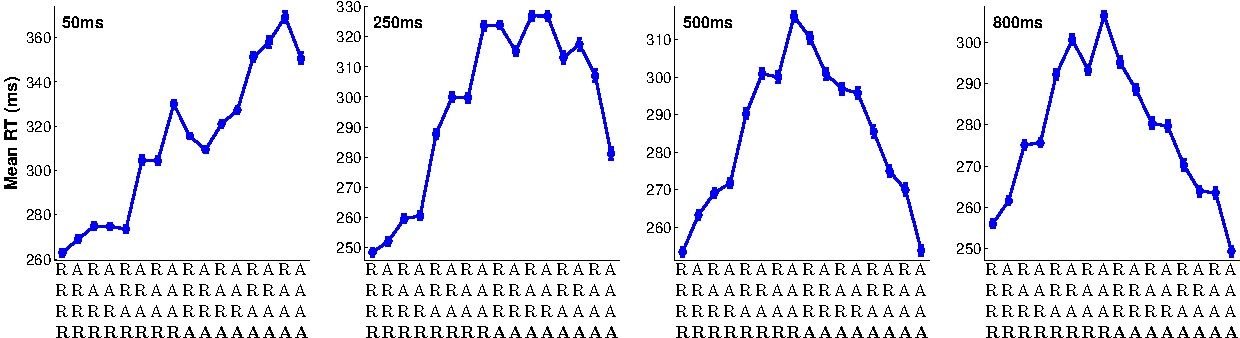
\includegraphics[width=1\textwidth]{rsi_scan.pdf}
\caption[Mean reaction time patterns as a function of RSI]{Reaction times averaged across all subjects performing a task with a particular RSI irrespective of experimental design. Note how reaction time results change from a cost-benefit pattern when the RSI is long (500 and 800ms subgroups) to a benefit-only pattern when the RSI is very short (50 ms). With a 250 ms RSI an intermediate pattern of results is observed. Error bars show the standard error of the mean.\label{rsi_scan}}
\end{figure}

\begin{figure}[t]
\centering
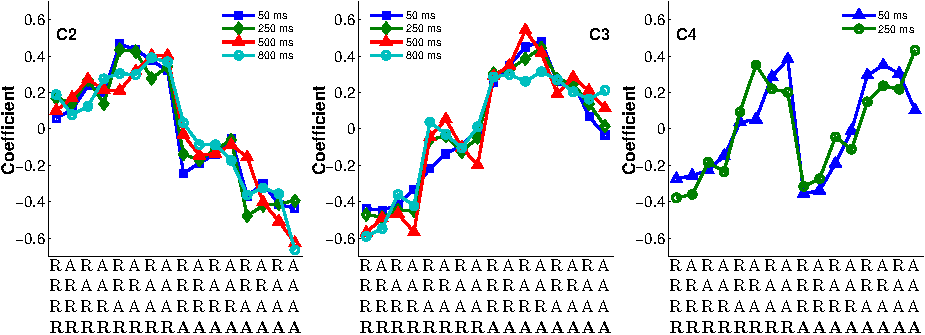
\includegraphics[width=1\textwidth]{components_rsi.pdf}
\caption[Invariance of the latent structure of sequential effects with RSI]{Invariance of the latent structure of sequential effects with RSI. Each panel shows the coefficient patterns of the equivalent component (from left to right: C2, C3 and C4) identified in four separate RSI subgroups - 50, 250, 500 and 800 ms - each including all subject which performed a task with a particular RSI irrespective of other experimental differences. Components significantly similar to C2 and C3 were identified in all all RSI subgroups, whereas a C4 anlogue was only identified in the 50 and 250 ms subgroups. The analysis performed in each subgroup was equal in every respect to that performed on the global pool of participants, i.e. PCA followed by an oblique rotation with the same targets. \label{components_rsi}}
\end{figure}

Assessing if and how the latent structure of sequential effects changes with RSI is of particular importance. In our data, there is a substantial difference across RSI in the sequential effects profile when averaged across subjects, as Figure~\ref{rsi_scan} shows. This is in keeping with the claim that  a ``benefit-only'' pattern is observed that is qualitatively different to the ``cost-benefit'' pattern that appears at long RSI values. \cite{Soetens85}. If this difference is reflected at the individual subject level, might expect a different latent variable structure to appear as a function of the RSI value. To test this hypothesis, we ran separate analyses for each RSI (50, 250, 500 and 800ms), identical in every respect to the main analyses apart from the restricted data sets. The results (omitting the uninteresting mean RT factor C1) are plotted in Figure~\ref{components_rsi}. Visual inspections suggests that these are essentially identical. To quantify this we computed the coefficient of congruence \cite{Gorsuch83} between components obtained in each subgroup and the corresponding global ones shown in Figure \ref{component_fits}. The significance of the coefficient of congruence values obtained was then estimated (see supplementary information for methodology). Components significantly similar to the global C2 and C3 ($p < 0.001$) were obtained in all RSI subgroups (see Figure \ref{components_rsi}, left and centre panel). Not only do the same two components C2 and C3 appear at all RSI values, the relative importance of these factors is roughly the same across RSI values: ignoring the contribution of global mean RT (i.e. C1) together they account for 71\%, 71\%, 61\% and 76\% of the variance respectively among the 50, 250, 500 and 800 ms subgroups. As for the fourth component, a component significantly similar to C4 was only found in the 50 and 250 ms subgroups. The 500 ms subgroup did produce a significant C4 at the $p < 0.05$ significance level, but this component showed a coefficient pattern that was visibly distorted relative to the global C4, suggesting that this component plays a role only at very short RSI values. Overall, this evidence suggests that C4 is only present at small RSI values.


\subsection{What does the C4 component mean?}

The previous discussion mirrors earlier work suggesting suggesting that the C4 pattern only emerges at very short RSI values. Both the raw data shown in Figure \ref{melis_jentzsch} and the latent variable C4 show nearly-identical patterns on the left and right hand side of the sequential effects plot, indicating that this component is entirely independent of the most recently presented stimulus (i.e., the one that the participant is supposed to be responding to). The fact that this pattern only emerges at short RSI values presents an intriguing possibility: perhaps people sometimes fail to process the current stimulus at all. When that happens, the sequential effects profile should still show the same general pattern, but applied with respect to the stimulus history excluding the present item. For instance if the \stimulus{RRRA} sequence occurred but the final stimulus was not processed, people should respond as if the history were in fact \stimulus{RRR}.

In order to estimate the influence of C2 and C3 if the last event had not been processed ``time shifted'' versions of the two components (which we denote C2* and C3*) were constructed in the following manner: to begin with the first (oldest) stimulus is discarded by averaging over all relevant pairs of sequences (e.g. \stimulus{ARRR} and \stimulus{RRRR} average to \stimulus{RRR}). Each of the resulting sequences is now replicated for the case in which the next even is an \stimulus{R} and for when it is an \stimulus{A}. So, for instance, in the end the sequences \stimulus{RRRR} and {RRRA} have the same RT value associated with them. We then took a weighted linear combination of C2* and C3* and compared it to C4. The results are shown in the left hand panel of Figure \ref{fits_4back}, and shows a reasonably good fit. In fact, a very similar result can be obtained using raw data. In the right hand panel of Figure \ref{fits_4back} we constructed time-shifted versions of the S-LRP and LRP-R signals and compared those to the RT data in \citeA{Jentzsch02}. Again, the match is very good.\footnote{The relative weights of the two predictors were estimated numerically. For the first comparison we fit a linear combination  of the form $k + w_1 C2^*+ w_2 C3^*$: the best fitting parameter values were $k=3.7\times 10^{-4}$, $w_1 = -0.405$ and $w_2 = 0.448$. For the second comparison we fit the model $k + w_1 SLRP^* + w_2 LRPR*$ where SLRP* and LRPR*. In this case best fitting parameter values were $k = 526.3$, $w1 = -0.551$ and $w2 = 0.646$. Note that in both cases the best fit is obtained with  $w_2 \approx -w_1$.} Taken together, these results suggest that there are only two ``fundamental'' components to sequential effects (i.e. C2 and C3) but at short RSI values people do not fully process the stimulus that has most recently been presented, which shows up as a ``residual'' component C4 that is in fact a combination of C2 and C3 applied to the stimulus history preceding the current trial.


\begin{figure}[t]
\centering
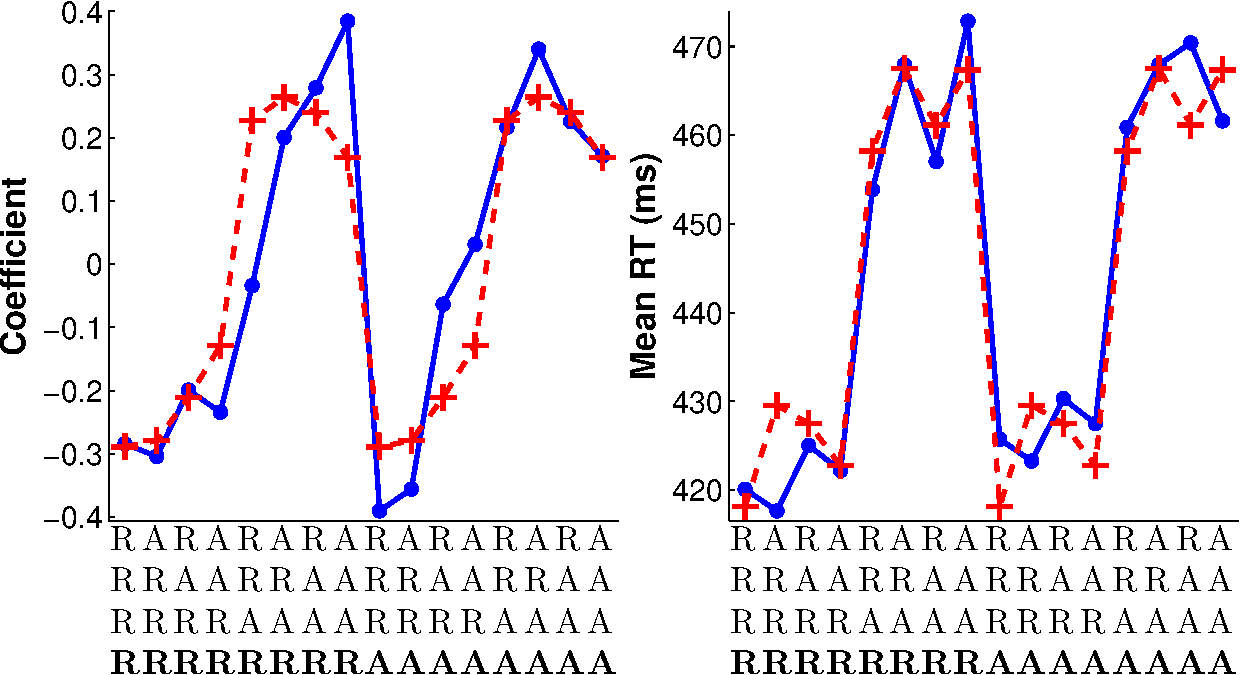
\includegraphics[width=.7\textwidth]{fits_4back.pdf}
\caption[C4 as the consequence of delayed activation of C2 and C3]{Relating C4 to C2 and C3. In the left panel, we plot the estimated component C4 (solid blue lines) against a weighted combination of C2* and C3* (dashed red line), where C2* and C3* are the ``time shifted'' version of C2 (see main text for details). In the right panel, a similar exercise is undertaken using raw data. The solid blue line in this plot shows the RT data from \protect\citeA{Jentzsch02}, and the dashed red line is a weighted combination of the time-shifted ERP data (i.e., S-LRP* and LRP-R*). $R^2$ values are 0.81 and 0.93 for the fits shown on the left and right panels respectively.}\label{fits_4back}
\end{figure}

\subsection{Individual differences}

\begin{figure}[t]
\centering
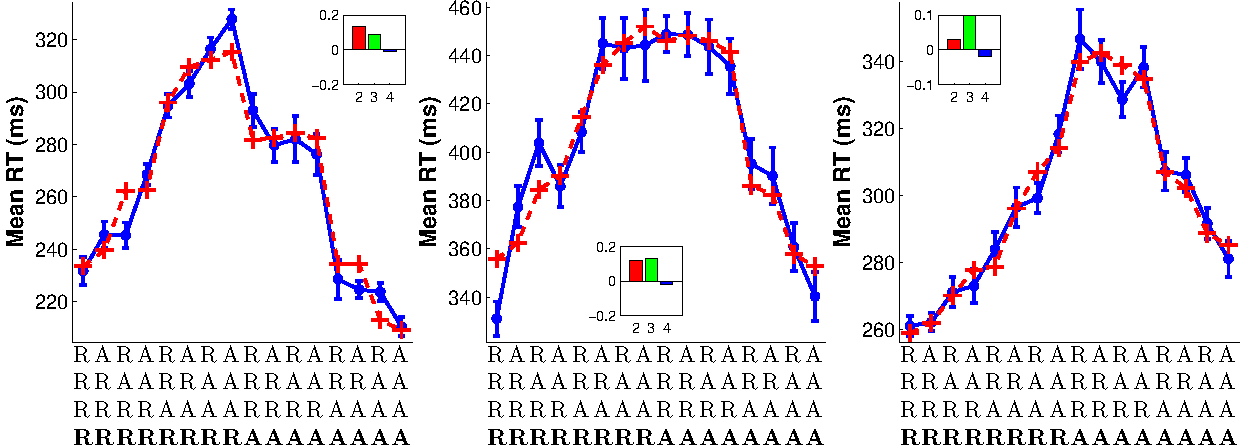
\includegraphics[width=1\textwidth]{typical.pdf}
\caption[Effect of varying the balance of C2 and C3]{Effect of varying the relative balance of C2 and C3, both with positive scores and when C4 is absent. Solid blue lines - individual participants included in our experiments chosen for illustration purposes. Dashed red lines - best fitting linear combinations of the form $s_1C1 + s_2C2 + s_3C3 + s_4C4$ where the $s_i$ are linear coefficients which we refer to as `scores' (see main text); the $C_i$ are the coefficient patterns of first four components. The range of results shown is characteristic of individual differences observed in experiments conducted with a relatively long RSI. Inset plots show the scores on C2, C3 and C4. Error bars show the standard error of the mean.\label{typical_subjects}}
\end{figure}

As the previous discussion illustrates, individual sequential effect patterns vary in terms of the relative contribution of the three components C2, C3 and C4, the last of which is arguably caused by the failure to fully process the presented stimulus when RSI is very short. What does this mean in terms of the patterns of sequential effects that are actually possible? The results of each individual can be represented by a point in `sequential effects space', the axes of which correspond to the scores on C2, C3 and C4.\footnotemark{} This three-dimensional space has eight octants corresponding to all possible combinations of sign of the three components. However, only half of the space is used, since C4 is always positive or close to zero. In order to clarify the effect of the three components we will analyze three cases separately: firstly we will look at the effects of varying C2 and C3 both with positive scores, and C4 held at zero; secondly, we will see the effect of allowing negative scores on C2 and C3 while still holding C4 at zero; finally,  the effect of C4 will be illustrated.

\footnotetext{See supplementary information for a plot of all individual scores.}

A balanced score on both C2 and C3 produces results similar to the cost-benefit pattern of sequential effects (see Figure \ref{typical_subjects}, central panel). A higher score on C2 relative to C3 induces a preference for alternations (see Figure \ref{typical_subjects}, left panel), whereas a higher score on C3 induces a repetition bias (see Figure \ref{typical_subjects}, right panel). Results from experiments conducted with a long RSI tend to fall along this range of scenarios \cite{Soetens85,Cho02,Jones02,Gokaydin11}, which can be described as a cost-benefit pattern with either a repetition or alternation bias.

\begin{figure}[t]
\centering
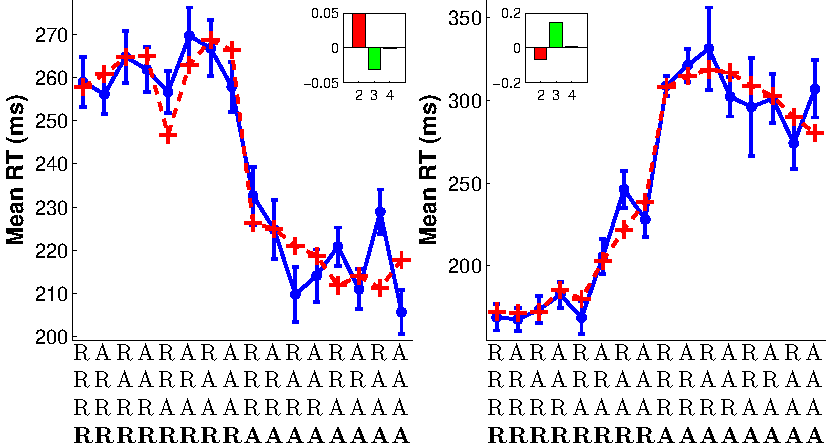
\includegraphics[width=.7\textwidth]{negative.pdf}
\caption[Effect of negative scores on C2 and C3]{Effect of allowing negative scores on C2 and C3, with C4 absent. Solid blue lines depict individual participants included in our experiments chosen for illustration purposes. Dashed red lines, best fitting linear combinations of the latent components C1-C4. Note how scores on C2 and C3 similar in magnitude and opposite in sign tend to produce patterns which may be mistaken for a two-tiered dependence on the last event and whether it was a repetition or an alternation; whether alternations or repetitions are faster depends on which component has a negative (or positive) score. Inset plots show scores on C2, C3 and C4. Error bars show the standard error of the mean.}\label{negative_subjects}
\end{figure}

Allowing the sign of the score on either C2 or C3 to go negative while still holding C4 at zero produces results no longer recognizable as a cost-benefit pattern. In particular, when the scores on C2 and C3 are approximately equal in magnitude but opposite in sign the resulting pattern resembles a two-tiered dependence on the last event (see Figure \ref{negative_subjects}), with faster reaction time to repetitions or alternations depending on whether C2 or C3 has a higher score. It is interesting to note that, if viewed in isolation, the patterns shown in Figure \ref{negative_subjects} would likely be interpreted as a trivial dependence on the last event, when in fact they are the product of a combination of two complex looking patterns. Only one individual participant was found to have a strong negative score on both C2 and C3, which may point to constraints on the allowed combinations of the two components. However, the good qualitative fit to the said subject indicates that it may be possible -- yet rare -- for both C2 and C3 to be negative. Finally it is worth mentioning that the contribution of a component with a negative score, when looked at in terms of its coefficient pattern, is an `upside-down' version of what can be seen in Figure \ref{component_fits}; this raises some conceptual issues which are discussed in detail below.

\begin{figure}[t]
\centering
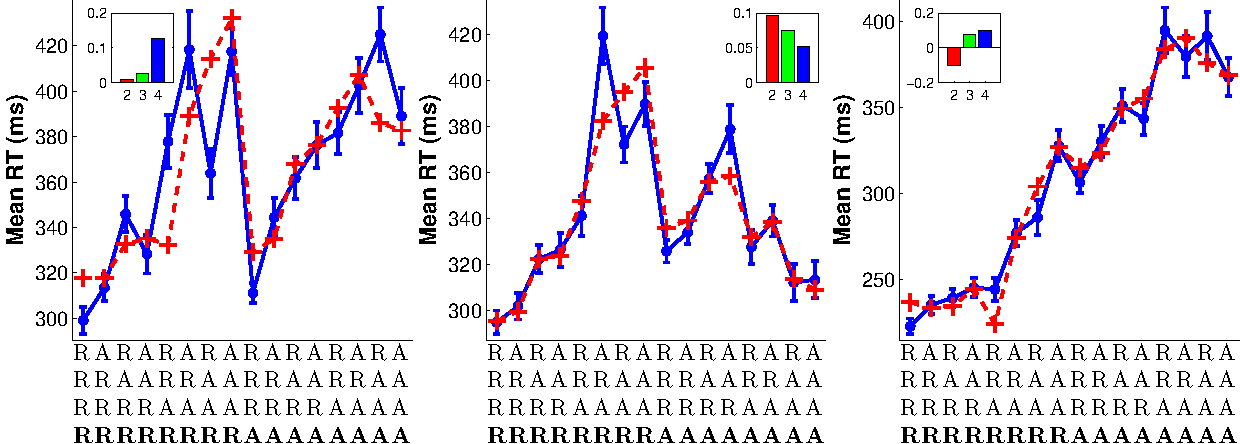
\includegraphics[width=1\textwidth]{c4.pdf}
\caption[The effect of C4]{The effect of C4. Solid blue lines show individual participants included in our experiments chosen for illustration purposes. Dashed red lines show best fitting linear combinations C1-C4. The left panel shows an individual displaying results similar to C4 in isolation; the middle panel shows a pattern of sequential effects not described before but which is displayed by several individuals; the right panel shows an individual exhibiting a typical benefit-only type of result. Inset plots show scores on C2, C3 and C4. Error bars show the standard error of the mean.} \label{c4_effect}
\end{figure}

The influence of C4 is only felt when the RSI is short, under which conditions it sometimes manifests itself in relative isolation,  i.e. with little contribution from either C2 or C3 (Figure \ref{c4_effect}, left panel). However, C4 is also necessary, in combination with C2 and C3, to explain other patterns of results, some of which were not described before in the literature (Figure \ref{c4_effect}, middle panel). Perhaps more importantly, C4 is also necessary in order to explain the the benefit-only pattern of sequential effects, often observed at an individual level when the RSI short (Figure \ref{c4_effect}, right panel). Note that all three individuals shown in Figure \ref{c4_effect} come from experiments conducted with a 50 ms RSI. Finally, no single individual exhibited a strong negative score on C4 so it not known whether this component can change sign in the same way as C2 and C3 can.



\section{Discussion}

Our main finding is that across different experimental conditions, as well as for different individuals performing the same experiment, the patterns of sequential effects vary in a limited number of ways. There appear to be only two fundamental dimensions upon which individual sequential effect patterns can vary, which we have tentatively linked to C2 and C3, plus the rarer C4 dimension which itself appears to be reducible to C2 and C3 under the assumption that the most recent stimulus has not been properly processed at the time the response is given (explaining why it appears only at short RSI values). A corollary of our results is that individual differences are confirmed as meaningful are not merely due to noise.


\subsection{The nature of sequential effects: C2 and C3}

The PCA results indicate the presence of two main components responsible for sequential effects. On the other hand, previous empirical evidence points to the existence of two separate processing stages involved in sequential effects, one pre-motor in origin and related to stimuli, and the other motoric and related to responses. It stands to reason that latent components and processing stages might be related, and in this spirit an attempt was made to map the coefficient patterns of the two latent variables (C2 and C3) to the best evidence available about the relative contributions of the two processing stages, namely S-LRP and LRP-R (see Figure \ref{component_fits}). The similarities encountered are consistent with the proposed relationship but fall short of providing conclusive evidence that the latent variables C2 and C3 do in fact reflect the separate processing of stimuli and responses. Nevertheless, although some caution is warranted, the implications of such a relationship are worth considering.

Recall that S-LRP and LRP-R are time measurements. One possibility then is that C2 and C3 simply reflect the time that it takes to process stimuli and responses in a serial fashion. However, this view clashes with the fact that the C2 and C3 can have a negative score, implying a negative processing time. A more nuanced view would be to consider that C2 and C3 reflect different signals related the separate processing of stimuli and responses. Note that while S-LRP and LRP-R have time units, they were measured with respect to a point defined by a threshold amplitude of the LRP. What this means is that S-LRP and LRP-R might reflect the \textit{amplitude} of different signals rather than simply processing times. If we take this view it becomes easier to accept that C2 and C3 might become negative, as this may possibly reflect a negative contribution of corresponding neurological signals towards reaction times.

One recent suggestion in the literature is that S-LRP and LRP-R reflect the tracking of different statistics about the environment \cite{Jones13} and, inasmuch a relationship between S-LRP/LRP-R and C2/C3  holds, this would imply the latent components also reflect different statistics. However, we again stumble on the fact that C2 and C3 can have a negative sign, implying that under some circumstances subjects would be tracking some form of inverse statistics, something which makes little sense from a computational point of view. When the RSI is long, both C2 and C3 are almost always positive, in which case a computational interpretation of the latent components may be possible. In fact, it has been argued that the cost-benefit pattern of sequential effects approximates the computations of an ideal observer \cite{Yu08}. However, it seems that the full range of different sequential effects, and in particular those observed with a short RSI, might only be explainable at a process level. The possible role of processing constraints in the results observed when the RSI is short, and in particular the emergence of C4, is discussed below.

A final possibility is that C2 and C3 play the role of separate detectors of repeating and alternating patterns in the sequence. Several authors have argued in the past for the need to postulate independent mechanisms in charge of detecting repetitions and alternations \cite{Hale69,Maloney05}. This theory fits with the symmetry observed in the coefficient patterns of C2 and C3, which implies that C2 and C3 have similar roles but applied to alternations and repetitions respectively. Finally, since higher coefficient values imply slower reaction times, in this view C2 would play the role of an alternation detector and C3 that of a repetition detector.

Irrespective of computational interpretations, there are some clues as to the mechanisms underlying sequential effects. In particular, there is a considerable evidence for the role of a geometric weighted average of the previous sequence, also known as exponential filter, in sequential effects \cite<e.g.>{Laming69,Yu08,Jones13}. Interestingly, an exponential filter of the sequence of stimuli produces a pattern of results with a remarkable degree of similarity with LRP-R (now shown), and it has in fact been argued that the two are related \cite{Jones13}. By proposing a correspondence between LRP-R and C3, it is further implied that this component might reflect an exponential filter of the sequence.

The mechanism behind S-LRP is less well understood, partly because it displays a strong alternation bias (i.e. faster RT to alternations), a seemingly simple feature which has nevertheless been notoriously hard to reproduce \cite{Wilder09,Jones13}. Some authors suggest that S-LRP corresponds to a second type of exponential filter, one which is applied to the sequence of repetitions and alternations rather than individual stimuli \cite{Jones13}. However, such a filter produces a pattern of results with no alternation or repetition bias (not shown), and in order to reproduce the alternation bias of S-LRP it has been necessary to postulate an additional mechanism \cite{Jones13}. So while the role of an exponential filter in generating a component looking like LRP-R seems well established, the mechanism behind S-LRP is not as well understood, and the same conclusions apply to the latent components C2 and C3 insofar as they correspond to S-LRP and LRP-R respectively.

\subsection{The role of processing speed: C4}

Crucial to understanding the nature of C4 is a study which contrasted sequential effects in young (ages between 19 and 25 years) and elderly (ages between 60 and 75 years) subjects \cite{Melis02}. When performing a 2AFC with a long RSI (1000 ms) there was little difference between the two groups except that the elderly participants were slower overall. However, when performing the same task with a 50 ms RSI, results were markedly different: the young group produced a benefit-only pattern typical of experiments with a short RSI (see Figure \ref{rsi_scan}, left panel); in contrast, the elderly group displayed a dependence on the second-to-last event (see Figure \ref{melis_jentzsch}) which we now know is related to C4. \citeA{Melis02} suggest that the underlying variable responsible for the differences observed between young and elderly groups is speed of processing, of which age is only a close correlate.

Speed of processing as a factor in sequential effects is compatible with the view of C4 as residual activation of C2 and C3 from the previous time step discussed above: a processing delay could in principle lead to a greater overlap between the activation at time step $t-1$ and that at time $t$. This interference between adjacent events would only be felt with a short RSI, when pressure on processing capacity is maximal. Regrettably, information on the age of participants was not collected for this study, something which would have allowed and investigation of the relationship between C4 score and age. Nevertheless, the vast majority of the subjects in this study were first year psychology students with a modal age of 18 years. It is therefore highly unlikely that processing speed limitations due to age played a role in the experiments reported here.

Finally, age might not be the only factor influencing processing speed. A second experiment which produced a pattern similar to C4 was conducted in subjects with a mean age of 27.4 years \cite{Jentzsch02}. It is unlikely that processing speed would have been limiting at such a relatively young age. However, the experiment in question was an unusually long version of a 2AFC both in terms of total number of trials (3960) and number of trials per block (330), more than twice the length of most 2AFCs \cite{Soetens85,Cho02,Jones02} as well as of our own experiments. Fatigue could therefore also play a role, possibly via a saturation effect and resulting decrease in processing speed. More work is necessary in order to establish the role of processing speed and/or fatigue in sequential effects. Just as the trajectory of the mean scores on C2, C3 and C4 as the RSI is varied was investigated here, it is important to do the same when varying age and the length of the experiment.

\subsection{Conclusion}

This work establishes a unified framework for understanding sequential effects. A latent structure was identified consisting of two main components and a minor one. A mapping was proposed between the two main components of sequential effects and the separate processing of stimuli and of responses. Further, the possibility was discussed that the minor component is a consequence of processing constraints when the response-stimulus interval is very short. Irrespective of the interpretation of the latent components, this work provides a unified descriptive model of a wide range of types of sequential effects, allowing for a clearer contextualization of past and future experimental results. Finally, the results presented here may carry more general implications for the mechanisms underlying human pattern detection, both at a psychological and neurophysiological level.

%\bibliographystyle{apacite}
%\bibdata{additional}
%\bibliography{zotero_library}


\begin{thebibliography}{}

\bibitem [\protect \citeauthoryear {%
Arons%
\ \BBA {} Irwin%
}{%
Arons%
\ \BBA {} Irwin%
}{%
{\protect \APACyear {1932}}%
}]{%
Arons32}
\APACinsertmetastar {%
Arons32}%
\begin{APACrefauthors}%
Arons, L.%
\BCBT {}\ \BBA {} Irwin, F\BPBI W.%
\end{APACrefauthors}%
\unskip\
\newblock
\APACrefYearMonthDay{1932}{}{}.
\newblock
{\BBOQ}\APACrefatitle {Equal weights and psychophysical judgments.} {Equal
  weights and psychophysical judgments.}{\BBCQ}
\newblock
\APACjournalVolNumPages{Journal of Experimental Psychology}{15}{6}{733--751}.
\PrintBackRefs{\CurrentBib}

\bibitem [\protect \citeauthoryear {%
Bertelson%
}{%
Bertelson%
}{%
{\protect \APACyear {1961}}%
}]{%
Bertelson61}
\APACinsertmetastar {%
Bertelson61}%
\begin{APACrefauthors}%
Bertelson, P.%
\end{APACrefauthors}%
\unskip\
\newblock
\APACrefYearMonthDay{1961}{}{}.
\newblock
{\BBOQ}\APACrefatitle {Sequential redundancy and speed in a serial two-choice
  responding task} {Sequential redundancy and speed in a serial two-choice
  responding task}.{\BBCQ}
\newblock
\APACjournalVolNumPages{Quarterly Journal of Experimental
  Psychology}{13}{2}{90--102}.
\PrintBackRefs{\CurrentBib}

\bibitem [\protect \citeauthoryear {%
Bertelson%
}{%
Bertelson%
}{%
{\protect \APACyear {1965}}%
}]{%
Bertelson65}
\APACinsertmetastar {%
Bertelson65}%
\begin{APACrefauthors}%
Bertelson, P.%
\end{APACrefauthors}%
\unskip\
\newblock
\APACrefYearMonthDay{1965}{}{}.
\newblock
{\BBOQ}\APACrefatitle {Serial Choice Reaction-time as a Function of Response
  versus Signal-and-Response Repetition} {Serial choice reaction-time as a
  function of response versus signal-and-response repetition}.{\BBCQ}
\newblock
\APACjournalVolNumPages{Nature}{206}{4980}{217--218}.
\PrintBackRefs{\CurrentBib}

\bibitem [\protect \citeauthoryear {%
Cho%
\ \protect \BOthers {.}}{%
Cho%
\ \protect \BOthers {.}}{%
{\protect \APACyear {2002}}%
}]{%
Cho02}
\APACinsertmetastar {%
Cho02}%
\begin{APACrefauthors}%
Cho, R\BPBI Y.%
, Nystrom, L\BPBI E.%
, Brown, E\BPBI T.%
, Jones, A\BPBI D.%
, Braver, T\BPBI S.%
, Holmes, P\BPBI J.%
\BCBL {}\ \BBA {} Cohen, J\BPBI D.%
\end{APACrefauthors}%
\unskip\
\newblock
\APACrefYearMonthDay{2002}{}{}.
\newblock
{\BBOQ}\APACrefatitle {Mechanisms underlying dependencies of performance on
  stimulus history in a two-alternative forced-choice task} {Mechanisms
  underlying dependencies of performance on stimulus history in a
  two-alternative forced-choice task}.{\BBCQ}
\newblock
\APACjournalVolNumPages{Cognitive, Affective, \& Behavioral
  Neuroscience}{4}{2}{283--299}.
\PrintBackRefs{\CurrentBib}

\bibitem [\protect \citeauthoryear {%
Fabrigar%
, Wegener%
, MacCallum%
\BCBL {}\ \BBA {} Strahan%
}{%
Fabrigar%
\ \protect \BOthers {.}}{%
{\protect \APACyear {1999}}%
}]{%
fabrigar1999evaluating}
\APACinsertmetastar {%
fabrigar1999evaluating}%
\begin{APACrefauthors}%
Fabrigar, L\BPBI R.%
, Wegener, D\BPBI T.%
, MacCallum, R\BPBI C.%
\BCBL {}\ \BBA {} Strahan, E\BPBI J.%
\end{APACrefauthors}%
\unskip\
\newblock
\APACrefYearMonthDay{1999}{}{}.
\newblock
{\BBOQ}\APACrefatitle {Evaluating the use of exploratory factor analysis in
  psychological research.} {Evaluating the use of exploratory factor analysis
  in psychological research.}{\BBCQ}
\newblock
\APACjournalVolNumPages{Psychological methods}{4}{3}{272-299}.
\PrintBackRefs{\CurrentBib}

\bibitem [\protect \citeauthoryear {%
Falmagne%
}{%
Falmagne%
}{%
{\protect \APACyear {1965}}%
}]{%
Falmagne65}
\APACinsertmetastar {%
Falmagne65}%
\begin{APACrefauthors}%
Falmagne, J.%
\end{APACrefauthors}%
\unskip\
\newblock
\APACrefYearMonthDay{1965}{}{}.
\newblock
{\BBOQ}\APACrefatitle {Stochastic models for choice reaction time with
  applications to experimental results} {Stochastic models for choice reaction
  time with applications to experimental results}.{\BBCQ}
\newblock
\APACjournalVolNumPages{Journal of Mathematical Psychology}{2}{1}{77--124}.
\PrintBackRefs{\CurrentBib}

\bibitem [\protect \citeauthoryear {%
Fernberger%
}{%
Fernberger%
}{%
{\protect \APACyear {1920}}%
}]{%
Fernberger20}
\APACinsertmetastar {%
Fernberger20}%
\begin{APACrefauthors}%
Fernberger, S\BPBI W.%
\end{APACrefauthors}%
\unskip\
\newblock
\APACrefYearMonthDay{1920}{}{}.
\newblock
{\BBOQ}\APACrefatitle {Interdependence of judgments within the series for the
  method of constant stimuli.} {Interdependence of judgments within the series
  for the method of constant stimuli.}{\BBCQ}
\newblock
\APACjournalVolNumPages{Journal of Experimental Psychology}{3}{2}{126}.
\PrintBackRefs{\CurrentBib}

\bibitem [\protect \citeauthoryear {%
Gilovich%
, Vallone%
\BCBL {}\ \BBA {} Tversky%
}{%
Gilovich%
\ \protect \BOthers {.}}{%
{\protect \APACyear {1985}}%
}]{%
Gilovich85}
\APACinsertmetastar {%
Gilovich85}%
\begin{APACrefauthors}%
Gilovich, T.%
, Vallone, R.%
\BCBL {}\ \BBA {} Tversky, A.%
\end{APACrefauthors}%
\unskip\
\newblock
\APACrefYearMonthDay{1985}{{\APACmonth{07}}}{}.
\newblock
{\BBOQ}\APACrefatitle {The hot hand in basketball: On the misperception of
  random sequences} {The hot hand in basketball: On the misperception of random
  sequences}.{\BBCQ}
\newblock
\APACjournalVolNumPages{Cognitive Psychology}{17}{3}{295--314}.
\PrintBackRefs{\CurrentBib}

\bibitem [\protect \citeauthoryear {%
Gokaydin%
, Ma-Wyatt%
, Navarro%
\BCBL {}\ \BBA {} Perfors%
}{%
Gokaydin%
\ \protect \BOthers {.}}{%
{\protect \APACyear {2011}}%
}]{%
Gokaydin11}
\APACinsertmetastar {%
Gokaydin11}%
\begin{APACrefauthors}%
Gokaydin, D.%
, Ma-Wyatt, A\BPBI M.%
, Navarro, D\BPBI J.%
\BCBL {}\ \BBA {} Perfors, A\BPBI F.%
\end{APACrefauthors}%
\unskip\
\newblock
\APACrefYearMonthDay{2011}{}{}.
\newblock
{\BBOQ}\APACrefatitle {Humans use different statistics for sequence analysis
  depending on the task} {Humans use different statistics for sequence analysis
  depending on the task}.{\BBCQ}
\newblock
\BIn{} \APACrefbtitle {Annual Meeting of the Cognitive Science Society (33rd:
  2011: Boston, {USA}) {CogSci} 2011.} {Annual meeting of the cognitive science
  society (33rd: 2011: Boston, {USA}) {CogSci} 2011.}
\PrintBackRefs{\CurrentBib}

\bibitem [\protect \citeauthoryear {%
Gorsuch%
}{%
Gorsuch%
}{%
{\protect \APACyear {1983}}%
}]{%
Gorsuch83}
\APACinsertmetastar {%
Gorsuch83}%
\begin{APACrefauthors}%
Gorsuch, R\BPBI L.%
\end{APACrefauthors}%
\unskip\
\newblock
\APACrefYear{1983}.
\newblock
\APACrefbtitle {Factor analysis} {Factor analysis}.
\newblock
\APACaddressPublisher{Hillsdale, N.J.}{L. Erlbaum Associates}.
\PrintBackRefs{\CurrentBib}

\bibitem [\protect \citeauthoryear {%
D.~Hale%
}{%
D.~Hale%
}{%
{\protect \APACyear {1969}}%
}]{%
Hale69}
\APACinsertmetastar {%
Hale69}%
\begin{APACrefauthors}%
Hale, D.%
\end{APACrefauthors}%
\unskip\
\newblock
\APACrefYearMonthDay{1969}{}{}.
\newblock
{\BBOQ}\APACrefatitle {Repetition and probability effects in a serial choice
  reaction task} {Repetition and probability effects in a serial choice
  reaction task}.{\BBCQ}
\newblock
\APACjournalVolNumPages{Acta Psychologica}{29}{}{163--171}.
\PrintBackRefs{\CurrentBib}

\bibitem [\protect \citeauthoryear {%
D\BPBI J.~Hale%
}{%
D\BPBI J.~Hale%
}{%
{\protect \APACyear {1967}}%
}]{%
Hale67}
\APACinsertmetastar {%
Hale67}%
\begin{APACrefauthors}%
Hale, D\BPBI J.%
\end{APACrefauthors}%
\unskip\
\newblock
\APACrefYearMonthDay{1967}{}{}.
\newblock
{\BBOQ}\APACrefatitle {Sequential effects in a two-choice serial reaction task}
  {Sequential effects in a two-choice serial reaction task}.{\BBCQ}
\newblock
\APACjournalVolNumPages{The Quarterly journal of experimental
  psychology}{19}{2}{133--141}.
\PrintBackRefs{\CurrentBib}

\bibitem [\protect \citeauthoryear {%
Hannes%
}{%
Hannes%
}{%
{\protect \APACyear {1968}}%
}]{%
Hannes68}
\APACinsertmetastar {%
Hannes68}%
\begin{APACrefauthors}%
Hannes, M.%
\end{APACrefauthors}%
\unskip\
\newblock
\APACrefYearMonthDay{1968}{}{}.
\newblock
{\BBOQ}\APACrefatitle {The Effect of Stimulus Repetitions and Alternations on
  One-Finger and Two-Finger Responding in Two-Choice Reaction Time} {The effect
  of stimulus repetitions and alternations on one-finger and two-finger
  responding in two-choice reaction time}.{\BBCQ}
\newblock
\APACjournalVolNumPages{The Journal of Psychology}{69}{2}{161--164}.
\PrintBackRefs{\CurrentBib}

\bibitem [\protect \citeauthoryear {%
Jarvik%
}{%
Jarvik%
}{%
{\protect \APACyear {1951}}%
}]{%
Jarvik51}
\APACinsertmetastar {%
Jarvik51}%
\begin{APACrefauthors}%
Jarvik, M\BPBI E.%
\end{APACrefauthors}%
\unskip\
\newblock
\APACrefYearMonthDay{1951}{}{}.
\newblock
{\BBOQ}\APACrefatitle {Probability learning and a negative recency effect in
  the serial anticipation of alternative symbols.} {Probability learning and a
  negative recency effect in the serial anticipation of alternative
  symbols.}{\BBCQ}
\newblock
\APACjournalVolNumPages{Journal of Experimental Psychology}{41}{4}{291--297}.
\PrintBackRefs{\CurrentBib}

\bibitem [\protect \citeauthoryear {%
Jentzsch%
\ \BBA {} Leuthold%
}{%
Jentzsch%
\ \BBA {} Leuthold%
}{%
{\protect \APACyear {2005}}%
}]{%
Jentzsch05}
\APACinsertmetastar {%
Jentzsch05}%
\begin{APACrefauthors}%
Jentzsch, I.%
\BCBT {}\ \BBA {} Leuthold, H.%
\end{APACrefauthors}%
\unskip\
\newblock
\APACrefYearMonthDay{2005}{}{}.
\newblock
{\BBOQ}\APACrefatitle {Response conflict determines sequential effects in
  serial response time tasks with short response-stimulus intervals} {Response
  conflict determines sequential effects in serial response time tasks with
  short response-stimulus intervals}.{\BBCQ}
\newblock
\APACjournalVolNumPages{Journal of experimental psychology. Human perception
  and performance}{31}{4}{731--748}.
\PrintBackRefs{\CurrentBib}

\bibitem [\protect \citeauthoryear {%
Jentzsch%
\ \BBA {} Sommer%
}{%
Jentzsch%
\ \BBA {} Sommer%
}{%
{\protect \APACyear {2002}}%
}]{%
Jentzsch02}
\APACinsertmetastar {%
Jentzsch02}%
\begin{APACrefauthors}%
Jentzsch, I.%
\BCBT {}\ \BBA {} Sommer, W.%
\end{APACrefauthors}%
\unskip\
\newblock
\APACrefYearMonthDay{2002}{}{}.
\newblock
{\BBOQ}\APACrefatitle {Functional localization and mechanisms of sequential
  effects in serial reaction time tasks} {Functional localization and
  mechanisms of sequential effects in serial reaction time tasks}.{\BBCQ}
\newblock
\APACjournalVolNumPages{Perception \& psychophysics}{64}{7}{1169--1188}.
\PrintBackRefs{\CurrentBib}

\bibitem [\protect \citeauthoryear {%
A\BPBI D.~Jones%
, Cho%
, Nystrom%
\BCBL {}\ \BBA {} Cohen%
}{%
A\BPBI D.~Jones%
\ \protect \BOthers {.}}{%
{\protect \APACyear {2002}}%
}]{%
Jones02}
\APACinsertmetastar {%
Jones02}%
\begin{APACrefauthors}%
Jones, A\BPBI D.%
, Cho, R\BPBI Y.%
, Nystrom, L\BPBI E.%
\BCBL {}\ \BBA {} Cohen, J\BPBI D.%
\end{APACrefauthors}%
\unskip\
\newblock
\APACrefYearMonthDay{2002}{}{}.
\newblock
{\BBOQ}\APACrefatitle {A computational model of anterior cingulate function in
  speeded response tasks: Effects of frequency, sequence, and conflict} {A
  computational model of anterior cingulate function in speeded response tasks:
  Effects of frequency, sequence, and conflict}.{\BBCQ}
\newblock
\APACjournalVolNumPages{Cognitive, Affective, \& Behavioral
  Neuroscience}{4}{2}{300--317}.
\PrintBackRefs{\CurrentBib}

\bibitem [\protect \citeauthoryear {%
M.~Jones%
, Curran%
, Mozer%
\BCBL {}\ \BBA {} Wilder%
}{%
M.~Jones%
\ \protect \BOthers {.}}{%
{\protect \APACyear {2013}}%
}]{%
Jones13}
\APACinsertmetastar {%
Jones13}%
\begin{APACrefauthors}%
Jones, M.%
, Curran, T.%
, Mozer, M\BPBI C.%
\BCBL {}\ \BBA {} Wilder, M\BPBI H.%
\end{APACrefauthors}%
\unskip\
\newblock
\APACrefYearMonthDay{2013}{}{}.
\newblock
{\BBOQ}\APACrefatitle {Sequential effects in response time reveal learning
  mechanisms and event representations} {Sequential effects in response time
  reveal learning mechanisms and event representations}.{\BBCQ}
\newblock
\APACjournalVolNumPages{Psychological review}{120}{3}{628--666}.
\PrintBackRefs{\CurrentBib}

\bibitem [\protect \citeauthoryear {%
Kirby%
}{%
Kirby%
}{%
{\protect \APACyear {1972}}%
}]{%
Kirby72}
\APACinsertmetastar {%
Kirby72}%
\begin{APACrefauthors}%
Kirby, N\BPBI H.%
\end{APACrefauthors}%
\unskip\
\newblock
\APACrefYearMonthDay{1972}{}{}.
\newblock
{\BBOQ}\APACrefatitle {Sequential effects of serial reaction time.} {Sequential
  effects of serial reaction time.}{\BBCQ}
\newblock
\APACjournalVolNumPages{Journal of Experimental Psychology}{96}{1}{32--36}.
\PrintBackRefs{\CurrentBib}

\bibitem [\protect \citeauthoryear {%
Kirby%
}{%
Kirby%
}{%
{\protect \APACyear {1976}}%
}]{%
Kirby76}
\APACinsertmetastar {%
Kirby76}%
\begin{APACrefauthors}%
Kirby, N\BPBI H.%
\end{APACrefauthors}%
\unskip\
\newblock
\APACrefYearMonthDay{1976}{}{}.
\newblock
{\BBOQ}\APACrefatitle {Sequential effects in an eight choice serial reaction
  time task using compatible and incompatible stimulus-response arrangements}
  {Sequential effects in an eight choice serial reaction time task using
  compatible and incompatible stimulus-response arrangements}.{\BBCQ}
\newblock
\APACjournalVolNumPages{Acta Psychologica}{40}{3}{207--216}.
\PrintBackRefs{\CurrentBib}

\bibitem [\protect \citeauthoryear {%
Kornblum%
}{%
Kornblum%
}{%
{\protect \APACyear {1969}}%
}]{%
Kornblum69}
\APACinsertmetastar {%
Kornblum69}%
\begin{APACrefauthors}%
Kornblum, S.%
\end{APACrefauthors}%
\unskip\
\newblock
\APACrefYearMonthDay{1969}{}{}.
\newblock
{\BBOQ}\APACrefatitle {Sequential determinants of information processing in
  serial and discrete choice reaction time.} {Sequential determinants of
  information processing in serial and discrete choice reaction time.}{\BBCQ}
\newblock
\APACjournalVolNumPages{Psychological Review}{76}{2}{113--131}.
\PrintBackRefs{\CurrentBib}

\bibitem [\protect \citeauthoryear {%
Laming%
}{%
Laming%
}{%
{\protect \APACyear {1968}}%
}]{%
Laming68}
\APACinsertmetastar {%
Laming68}%
\begin{APACrefauthors}%
Laming, D.%
\end{APACrefauthors}%
\unskip\
\newblock
\APACrefYear{1968}.
\newblock
\APACrefbtitle {Information theory of choice-reaction times.} {Information
  theory of choice-reaction times.}
\PrintBackRefs{\CurrentBib}

\bibitem [\protect \citeauthoryear {%
Laming%
}{%
Laming%
}{%
{\protect \APACyear {1969}}%
}]{%
Laming69}
\APACinsertmetastar {%
Laming69}%
\begin{APACrefauthors}%
Laming, D.%
\end{APACrefauthors}%
\unskip\
\newblock
\APACrefYearMonthDay{1969}{}{}.
\newblock
{\BBOQ}\APACrefatitle {Subjective probability in choice-reaction experiments}
  {Subjective probability in choice-reaction experiments}.{\BBCQ}
\newblock
\APACjournalVolNumPages{Journal of Mathematical Psychology}{6}{1}{81--120}.
\PrintBackRefs{\CurrentBib}

\bibitem [\protect \citeauthoryear {%
Leuthold%
, Sommer%
\BCBL {}\ \BBA {} Ulrich%
}{%
Leuthold%
\ \protect \BOthers {.}}{%
{\protect \APACyear {1996}}%
}]{%
Leuthold96}
\APACinsertmetastar {%
Leuthold96}%
\begin{APACrefauthors}%
Leuthold, H.%
, Sommer, W.%
\BCBL {}\ \BBA {} Ulrich, R.%
\end{APACrefauthors}%
\unskip\
\newblock
\APACrefYearMonthDay{1996}{}{}.
\newblock
{\BBOQ}\APACrefatitle {Partial advance information and response preparation:
  inferences from the lateralized readiness potential} {Partial advance
  information and response preparation: inferences from the lateralized
  readiness potential}.{\BBCQ}
\newblock
\APACjournalVolNumPages{Journal of experimental psychology.
  General}{125}{3}{307--323}.
\PrintBackRefs{\CurrentBib}

\bibitem [\protect \citeauthoryear {%
Maloney%
, Dal~Martello%
, Sahm%
\BCBL {}\ \BBA {} Spillmann%
}{%
Maloney%
\ \protect \BOthers {.}}{%
{\protect \APACyear {2005}}%
}]{%
Maloney05}
\APACinsertmetastar {%
Maloney05}%
\begin{APACrefauthors}%
Maloney, L\BPBI T.%
, Dal~Martello, M\BPBI F.%
, Sahm, C.%
\BCBL {}\ \BBA {} Spillmann, L.%
\end{APACrefauthors}%
\unskip\
\newblock
\APACrefYearMonthDay{2005}{}{}.
\newblock
{\BBOQ}\APACrefatitle {Past trials influence perception of ambiguous motion
  quartets through pattern completion} {Past trials influence perception of
  ambiguous motion quartets through pattern completion}.{\BBCQ}
\newblock
\APACjournalVolNumPages{Proceedings of the National Academy of Sciences of the
  United States of America}{102}{8}{3164--3169}.
\PrintBackRefs{\CurrentBib}

\bibitem [\protect \citeauthoryear {%
Melis%
, Soetens%
\BCBL {}\ \BBA {} van~der Molen%
}{%
Melis%
\ \protect \BOthers {.}}{%
{\protect \APACyear {2002}}%
}]{%
Melis02}
\APACinsertmetastar {%
Melis02}%
\begin{APACrefauthors}%
Melis, A.%
, Soetens, E.%
\BCBL {}\ \BBA {} van~der Molen, M\BPBI W.%
\end{APACrefauthors}%
\unskip\
\newblock
\APACrefYearMonthDay{2002}{}{}.
\newblock
{\BBOQ}\APACrefatitle {Process-Specific Slowing with Advancing Age: Evidence
  Derived from the Analysis of Sequential Effects} {Process-specific slowing
  with advancing age: Evidence derived from the analysis of sequential
  effects}.{\BBCQ}
\newblock
\APACjournalVolNumPages{Brain and Cognition}{49}{3}{420--435}.
\PrintBackRefs{\CurrentBib}

\bibitem [\protect \citeauthoryear {%
Nickerson%
}{%
Nickerson%
}{%
{\protect \APACyear {2002}}%
}]{%
Nickerson02}
\APACinsertmetastar {%
Nickerson02}%
\begin{APACrefauthors}%
Nickerson, R\BPBI S.%
\end{APACrefauthors}%
\unskip\
\newblock
\APACrefYearMonthDay{2002}{}{}.
\newblock
{\BBOQ}\APACrefatitle {The production and perception of randomness.} {The
  production and perception of randomness.}{\BBCQ}
\newblock
\APACjournalVolNumPages{Psychological Review}{109}{2}{330--357}.
\PrintBackRefs{\CurrentBib}

\bibitem [\protect \citeauthoryear {%
Ratcliff%
}{%
Ratcliff%
}{%
{\protect \APACyear {1993}}%
}]{%
Ratcliff93}
\APACinsertmetastar {%
Ratcliff93}%
\begin{APACrefauthors}%
Ratcliff, R.%
\end{APACrefauthors}%
\unskip\
\newblock
\APACrefYearMonthDay{1993}{}{}.
\newblock
{\BBOQ}\APACrefatitle {Methods for dealing with reaction time outliers}
  {Methods for dealing with reaction time outliers}.{\BBCQ}
\newblock
\APACjournalVolNumPages{Psychological bulletin}{114}{3}{510--532}.
\PrintBackRefs{\CurrentBib}

\bibitem [\protect \citeauthoryear {%
Remington%
}{%
Remington%
}{%
{\protect \APACyear {1969}}%
}]{%
Remington69}
\APACinsertmetastar {%
Remington69}%
\begin{APACrefauthors}%
Remington, R\BPBI J.%
\end{APACrefauthors}%
\unskip\
\newblock
\APACrefYearMonthDay{1969}{}{}.
\newblock
{\BBOQ}\APACrefatitle {Analysis of sequential effects on choice reaction
  times.} {Analysis of sequential effects on choice reaction times.}{\BBCQ}
\newblock
\APACjournalVolNumPages{Journal of Experimental Psychology}{82}{2}{250--257}.
\PrintBackRefs{\CurrentBib}

\bibitem [\protect \citeauthoryear {%
{SAS Institute Inc.}%
}{%
{SAS Institute Inc.}%
}{%
{\protect \APACyear {2010}}%
}]{%
SAS2010}
\APACinsertmetastar {%
SAS2010}%
\begin{APACrefauthors}%
{SAS Institute Inc.}%
\end{APACrefauthors}%
\unskip\
\newblock
\APACrefYear{2010}.
\newblock
\APACrefbtitle {{SAS/STAT} 9.22 User’s Guide} {{SAS/STAT} 9.22 user’s
  guide}.
\newblock
\APACaddressPublisher{Cary, NC}{SAS Institute Inc.}
\PrintBackRefs{\CurrentBib}

\bibitem [\protect \citeauthoryear {%
Schvaneveldt%
\ \BBA {} Chase%
}{%
Schvaneveldt%
\ \BBA {} Chase%
}{%
{\protect \APACyear {1969}}%
}]{%
Schvaneveldt69}
\APACinsertmetastar {%
Schvaneveldt69}%
\begin{APACrefauthors}%
Schvaneveldt, R\BPBI W.%
\BCBT {}\ \BBA {} Chase, W\BPBI G.%
\end{APACrefauthors}%
\unskip\
\newblock
\APACrefYearMonthDay{1969}{}{}.
\newblock
{\BBOQ}\APACrefatitle {Sequential effects in choice reaction time.} {Sequential
  effects in choice reaction time.}{\BBCQ}
\newblock
\APACjournalVolNumPages{Journal of Experimental Psychology}{80}{1}{1--8}.
\PrintBackRefs{\CurrentBib}

\bibitem [\protect \citeauthoryear {%
Soetens%
}{%
Soetens%
}{%
{\protect \APACyear {1998}}%
}]{%
Soetens98}
\APACinsertmetastar {%
Soetens98}%
\begin{APACrefauthors}%
Soetens, E.%
\end{APACrefauthors}%
\unskip\
\newblock
\APACrefYearMonthDay{1998}{}{}.
\newblock
{\BBOQ}\APACrefatitle {Localizing sequential effects in serial choice reaction
  time with the information reduction procedure.} {Localizing sequential
  effects in serial choice reaction time with the information reduction
  procedure.}{\BBCQ}
\newblock
\APACjournalVolNumPages{Journal of Experimental Psychology: Human Perception
  and Performance}{24}{2}{547}.
\PrintBackRefs{\CurrentBib}

\bibitem [\protect \citeauthoryear {%
Soetens%
, Boer%
\BCBL {}\ \BBA {} Hueting%
}{%
Soetens%
\ \protect \BOthers {.}}{%
{\protect \APACyear {1985}}%
}]{%
Soetens85}
\APACinsertmetastar {%
Soetens85}%
\begin{APACrefauthors}%
Soetens, E.%
, Boer, L\BPBI C.%
\BCBL {}\ \BBA {} Hueting, J\BPBI E.%
\end{APACrefauthors}%
\unskip\
\newblock
\APACrefYearMonthDay{1985}{}{}.
\newblock
{\BBOQ}\APACrefatitle {Expectancy or Automatic Facilitation? Separating
  Sequential Effects in Two-Choice Reaction Time} {Expectancy or automatic
  facilitation? separating sequential effects in two-choice reaction
  time}.{\BBCQ}
\newblock
\APACjournalVolNumPages{Journal of Experimental Psychology: Human Perception
  and Performance}{11}{5}{598--616}.
\PrintBackRefs{\CurrentBib}

\bibitem [\protect \citeauthoryear {%
Soetens%
, Deboeck%
\BCBL {}\ \BBA {} Hueting%
}{%
Soetens%
\ \protect \BOthers {.}}{%
{\protect \APACyear {1984}}%
}]{%
Soetens84}
\APACinsertmetastar {%
Soetens84}%
\begin{APACrefauthors}%
Soetens, E.%
, Deboeck, M.%
\BCBL {}\ \BBA {} Hueting, J.%
\end{APACrefauthors}%
\unskip\
\newblock
\APACrefYearMonthDay{1984}{}{}.
\newblock
{\BBOQ}\APACrefatitle {Automatic aftereffects in two-choice reaction time: a
  mathematical representation of some concepts} {Automatic aftereffects in
  two-choice reaction time: a mathematical representation of some
  concepts}.{\BBCQ}
\newblock
\APACjournalVolNumPages{Journal of experimental psychology. Human perception
  and performance}{10}{4}{581--598}.
\PrintBackRefs{\CurrentBib}

\bibitem [\protect \citeauthoryear {%
Sommer%
, Leuthold%
\BCBL {}\ \BBA {} Soetens%
}{%
Sommer%
\ \protect \BOthers {.}}{%
{\protect \APACyear {1999}}%
}]{%
Sommer99}
\APACinsertmetastar {%
Sommer99}%
\begin{APACrefauthors}%
Sommer, W.%
, Leuthold, H.%
\BCBL {}\ \BBA {} Soetens, E.%
\end{APACrefauthors}%
\unskip\
\newblock
\APACrefYearMonthDay{1999}{}{}.
\newblock
{\BBOQ}\APACrefatitle {Covert signs of expectancy in serial reaction time tasks
  revealed by event-related potentials} {Covert signs of expectancy in serial
  reaction time tasks revealed by event-related potentials}.{\BBCQ}
\newblock
\APACjournalVolNumPages{Perception \& psychophysics}{61}{2}{342--353}.
\PrintBackRefs{\CurrentBib}

\bibitem [\protect \citeauthoryear {%
Sommer%
, Matt%
\BCBL {}\ \BBA {} Leuthold%
}{%
Sommer%
\ \protect \BOthers {.}}{%
{\protect \APACyear {1990}}%
}]{%
Sommer90}
\APACinsertmetastar {%
Sommer90}%
\begin{APACrefauthors}%
Sommer, W.%
, Matt, J.%
\BCBL {}\ \BBA {} Leuthold, H.%
\end{APACrefauthors}%
\unskip\
\newblock
\APACrefYearMonthDay{1990}{}{}.
\newblock
{\BBOQ}\APACrefatitle {Consciousness of attention and expectancy as reflected
  in event-related potentials and reaction times} {Consciousness of attention
  and expectancy as reflected in event-related potentials and reaction
  times}.{\BBCQ}
\newblock
\APACjournalVolNumPages{Journal of experimental psychology. Learning, memory,
  and cognition}{16}{5}{902--915}.
\PrintBackRefs{\CurrentBib}

\bibitem [\protect \citeauthoryear {%
Squires%
, Wickens%
, Squires%
\BCBL {}\ \BBA {} Donchin%
}{%
Squires%
\ \protect \BOthers {.}}{%
{\protect \APACyear {1976}}%
}]{%
Squires76}
\APACinsertmetastar {%
Squires76}%
\begin{APACrefauthors}%
Squires, K\BPBI C.%
, Wickens, C.%
, Squires, N\BPBI K.%
\BCBL {}\ \BBA {} Donchin, E.%
\end{APACrefauthors}%
\unskip\
\newblock
\APACrefYearMonthDay{1976}{}{}.
\newblock
{\BBOQ}\APACrefatitle {The effect of stimulus sequence on the waveform of the
  cortical event-related potential} {The effect of stimulus sequence on the
  waveform of the cortical event-related potential}.{\BBCQ}
\newblock
\APACjournalVolNumPages{Science (New York, N.Y.)}{193}{4258}{1142--1146}.
\PrintBackRefs{\CurrentBib}

\bibitem [\protect \citeauthoryear {%
Vervaeck%
\ \BBA {} Boer%
}{%
Vervaeck%
\ \BBA {} Boer%
}{%
{\protect \APACyear {1980}}%
}]{%
Vervaeck80}
\APACinsertmetastar {%
Vervaeck80}%
\begin{APACrefauthors}%
Vervaeck, K\BPBI R.%
\BCBT {}\ \BBA {} Boer, L\BPBI C.%
\end{APACrefauthors}%
\unskip\
\newblock
\APACrefYearMonthDay{1980}{}{}.
\newblock
{\BBOQ}\APACrefatitle {Sequential effects in two-choice reaction time:
  Subjective expectancy and automatic after- effect at short response-stimulus
  intervals} {Sequential effects in two-choice reaction time: Subjective
  expectancy and automatic after- effect at short response-stimulus
  intervals}.{\BBCQ}
\newblock
\APACjournalVolNumPages{Acta Psychologica}{44}{2}{175--190}.
\PrintBackRefs{\CurrentBib}

\bibitem [\protect \citeauthoryear {%
M.~Wilder%
, Jones%
\BCBL {}\ \BBA {} Mozer%
}{%
M.~Wilder%
\ \protect \BOthers {.}}{%
{\protect \APACyear {2009}}%
}]{%
Wilder09}
\APACinsertmetastar {%
Wilder09}%
\begin{APACrefauthors}%
Wilder, M.%
, Jones, M.%
\BCBL {}\ \BBA {} Mozer, M\BPBI C.%
\end{APACrefauthors}%
\unskip\
\newblock
\APACrefYearMonthDay{2009}{}{}.
\newblock
{\BBOQ}\APACrefatitle {Sequential effects reflect parallel learning of multiple
  environmental regularities} {Sequential effects reflect parallel learning of
  multiple environmental regularities}.{\BBCQ}
\newblock
\BIn{} Y.~Bengio, D.~Schuurmans, J\BPBI D.~Lafferty, C\BPBI K\BPBI
  I.~Williams\BCBL {}\ \BBA {} A.~Culotta\ (\BEDS), \APACrefbtitle {Advances in
  Neural Information Processing Systems 22} {Advances in neural information
  processing systems 22}\ (\BPGS\ 2053--2061).
\newblock
\APACaddressPublisher{}{Curran Associates, Inc.}
\PrintBackRefs{\CurrentBib}

\bibitem [\protect \citeauthoryear {%
M\BPBI H.~Wilder%
, Jones%
, Ahmed%
, Curran%
\BCBL {}\ \BBA {} Mozer%
}{%
M\BPBI H.~Wilder%
\ \protect \BOthers {.}}{%
{\protect \APACyear {2013}}%
}]{%
Wilder13}
\APACinsertmetastar {%
Wilder13}%
\begin{APACrefauthors}%
Wilder, M\BPBI H.%
, Jones, M.%
, Ahmed, A\BPBI A.%
, Curran, T.%
\BCBL {}\ \BBA {} Mozer, M\BPBI C.%
\end{APACrefauthors}%
\unskip\
\newblock
\APACrefYearMonthDay{2013}{}{}.
\newblock
{\BBOQ}\APACrefatitle {The persistent impact of incidental experience} {The
  persistent impact of incidental experience}.{\BBCQ}
\newblock
\APACjournalVolNumPages{Psychonomic bulletin \& review}{}{}{}.
\PrintBackRefs{\CurrentBib}

\bibitem [\protect \citeauthoryear {%
Yu%
\ \BBA {} Cohen%
}{%
Yu%
\ \BBA {} Cohen%
}{%
{\protect \APACyear {2008}}%
}]{%
Yu08}
\APACinsertmetastar {%
Yu08}%
\begin{APACrefauthors}%
Yu, A\BPBI J.%
\BCBT {}\ \BBA {} Cohen, J\BPBI D.%
\end{APACrefauthors}%
\unskip\
\newblock
\APACrefYearMonthDay{2008}{}{}.
\newblock
{\BBOQ}\APACrefatitle {Sequential effects: Superstition or rational behavior?}
  {Sequential effects: Superstition or rational behavior?}{\BBCQ}
\newblock
\BIn{} D.~Koller, D.~Schuurmans, Y.~Bengio\BCBL {}\ \BBA {} L.~Bottou\ (\BEDS),
  \APACrefbtitle {Advances in Neural Information Processing Systems 21}
  {Advances in neural information processing systems 21}\ (\BPGS\ 1873--1880).
\newblock
\APACaddressPublisher{}{Curran Associates, Inc.}
\PrintBackRefs{\CurrentBib}

\end{thebibliography}

\end{document}
